% =============================================================================
%  Scale Without Support --- ICLR 2027 conference submission
%
%  PROVENANCE DISCIPLINE. Every numeric claim in this manuscript is followed by
%  a LaTeX comment naming the artifact it was read from. Nothing is estimated,
%  interpolated, or inferred. Claims the project's artifacts cannot support are
%  marked as such in the text, not silently omitted.
%
%  BUILD: latexmk -pdf main.tex   (needs only the files in this directory)
% =============================================================================
\documentclass{article}
\usepackage{iclr2027_conference,times}

\usepackage{amsmath,amssymb,amsthm}
\usepackage{booktabs}
\usepackage{multirow}
\usepackage{graphicx}
\usepackage{xcolor}
\usepackage[htt]{hyphenat}
\usepackage{tikz}
\usetikzlibrary{arrows.meta,positioning,calc,fit,backgrounds,shapes.geometric,
                decorations.pathreplacing,patterns}
\usepackage{pgfplots}
\pgfplotsset{compat=1.18}
\usepackage{hyperref}
\usepackage{url}


% ---------------------------------------------------------------- palette ---
% Okabe--Ito, colourblind-safe. Inherited unchanged from the project's own
% figure preamble so the reused TikZ sources compile without modification.
\definecolor{okBlue}   {HTML}{0072B2}
\definecolor{okVermil} {HTML}{D55E00}
\definecolor{okGreen}  {HTML}{009E73}
\definecolor{okOrange} {HTML}{E69F00}
\definecolor{okSky}    {HTML}{56B4E9}
\definecolor{okPurple} {HTML}{CC79A7}
\definecolor{okYellow} {HTML}{F0E442}
\definecolor{inkGrey}  {HTML}{4D4D4D}
\definecolor{softGrey} {HTML}{F2F2F2}

\tikzset{
  fignode/.style  = {rounded corners=2pt, draw, line width=0.6pt, align=center,
                     inner sep=4pt, font=\scriptsize},
  phase/.style    = {fignode, fill=okBlue!10, draw=okBlue, minimum width=26mm,
                     minimum height=9mm},
  corpus/.style   = {fignode, fill=okSky!18,  draw=okSky!90!black},
  artifact/.style = {fignode, fill=okGreen!12, draw=okGreen!90!black,
                     font=\scriptsize\ttfamily},
  finding/.style  = {fignode, fill=okVermil!12, draw=okVermil},
  failnode/.style = {fignode, fill=okVermil!18, draw=okVermil, line width=0.9pt},
  passnode/.style = {fignode, fill=okGreen!14, draw=okGreen!80!black, line width=0.9pt},
  evalnode/.style = {fignode, fill=okPurple!14, draw=okPurple!90!black},
  note/.style     = {align=left, font=\scriptsize\itshape, text=inkGrey, inner sep=2pt},
  grouplab/.style = {font=\scriptsize\bfseries, text=inkGrey},
  flow/.style     = {-{Stealth[length=4pt,width=3pt]}, draw=inkGrey, line width=0.7pt},
  weakflow/.style = {-{Stealth[length=4pt,width=3pt]}, draw=inkGrey!55,
                     line width=0.6pt, dashed},
  deadflow/.style = {-{Stealth[length=4pt,width=3pt]}, draw=okVermil,
                     line width=0.8pt, dash pattern=on 2pt off 1.6pt},
  edgelab/.style  = {font=\scriptsize, text=inkGrey, inner sep=1.5pt, fill=white,
                     rounded corners=1pt},
}

% ------------------------------------------------------------------ macros ---
\newcommand{\Sest}{\ensuremath{\widehat{S}}}
\newcommand{\Hest}{\ensuremath{\widehat{H}}}
\newcommand{\Strue}{\ensuremath{S}}
\newcommand{\Htrue}{\ensuremath{H}}
\newcommand{\arm}[1]{\texttt{#1}}
\newcommand{\ci}[2]{{\scriptsize$[#1,\,#2]$}}

\title{Scale Without Support: Fractal Signatures Are Not\\
Document Representations}

\author{}

%\iclrfinalcopy % Uncomment for camera-ready, NOT for submission.
\begin{document}
\maketitle

% =============================================================================
\begin{abstract}
A thermometer with a five-degree error bar can still resolve a half-degree
difference between two towns' \emph{climates} by averaging enough
single-day readings; it cannot tell you the temperature at one house on one
day, however sharp the average is. We argue the Hurst and H\"older
exponents used to fingerprint machine-generated text are exactly that kind
of instrument, and that this literature has read climate-level evidence as
an answer to the single-reading question. In signal-to-noise terms, the
exponent decomposes into a population term (signal) and estimator noise,
and at real document length noise swamps signal by more than an order of
magnitude. On $223{,}834$ GAGLE documents, $20$ of $20$ (domain, generator,
exponent) cells separate with non-overlapping $95\%$ intervals, confirmed
by a second, differently biased estimator agreeing on direction in $10$ of
$10$ H\"older cells --- the population term is real and reproducible.
Split each document's own tokens in half and re-estimate independently on
each half, and the flagship exponent agrees with itself at Spearman--Brown
$\rho=0.063$ against a $\rho\ge0.60$ bar fixed in advance, the best of
twenty candidate quantities reaching only $0.576$ --- almost none of that
signal survives to a single document. Four predictions follow, and all four
hold (Table~\ref{tab:map}): deleting all $54$ fractal features from an
$85$-feature detector leaves AUROC at $0.9984$ and TPR@$1\%$FPR
statistically unchanged ($0.9587\!\to\!0.9612$); a within-population task
holding the population term fixed by construction recovers only about a
sixth of the achievable signal; and the family pays only when the
population changes, $+0.0240$ AUROC on a matched RAID transfer --- the
population moving, not any document read more accurately. A second,
independent illusion appears in the same pipeline: a curvature detector's
paraphrase recall \emph{rises} to $0.63$--$0.86$ under attacks from models
sharing its scorer's lineage and collapses to $1.2$--$4.5\%$ once that
overlap is removed --- robustness the field would credit to the detector is
an artifact of who wrote the attack. The result is a condition, not a
theorem: treat a scaling estimator as a document-level representation only
once its split-half reliability at the deployment length clears the bar.
\end{abstract}

% =============================================================================
\section{Introduction}
\label{sec:intro}

Language has a fractal information structure: its per-token complexity is
self-similar across scales and long-range dependent, with a Hurst parameter near
$0.7$ \citep{alabdulmohsin2024fractal}. The observation extends to
generated text. \citet{alabdulmohsin2025tale} report that the H\"older and Hurst
exponents of natural language occupy a narrow band while those of language-model
output vary widely, and conclude that ``fractal parameters might prove helpful in
detecting LLM-generated text'' --- while declining to make the detection claim
themselves, on the grounds that the exponents describe processes rather than
documents. That caveat is usually read as a limitation of scope. We read it as a claim about
the object being measured, and we test it. A scaling exponent is defined by a limit
--- $R(n)/S(n)\sim n^{H}$ as $n\to\infty$ --- so every empirical use of one is an
estimator on a finite realisation, and whether it resolves anything about that
realisation, as opposed to the process that generated it, is a question about
support. Related work (Appendix~\ref{app:related}) reports no reliability
coefficient for a scaling estimator at document length.

\paragraph{The argument in one picture, before the notation.} A thermometer
with a five-degree error bar still resolves a real half-degree difference
between two towns' climates, once enough single-day readings are averaged
--- but handed one reading from one day, it cannot tell you which town
produced it, because the instrument's own noise is larger than the quantity
in question. Swap in a fractal exponent for the thermometer, a (domain,
generator) population for the town, and one document's token budget for the
single day, and this is the claim we test: the exponent's population-level
signal is real, but at the token budget an actual document supplies, the
exponent behaves like the one-day reading --- dominated by its own
estimation noise, not by anything specific to the document it was computed
from. \S\ref{sec:analogy} makes this literal, translates it into the
paper's notation term by term, and derives four falsifiable predictions
from it (Table~\ref{tab:map}); every technical result from here on is a
test of one of those four.

\paragraph{Two things this result is not.}
It is not an attack on a claim nobody made: the step from a distribution-level
separation to a per-document score is taken explicitly by the closest
neighbour of this work \citep{tulchinskii2023intrinsic}, a construction now
widespread as a detector
\citep{guo2026multiscale,west2025nonstationary,liu2026wavedetect,mansouri2026stability,teja2025pife,lacava2026luminol}
and as a characterisation of generated text
\citep{du2025correlation,yang2026turbulence}. Nor is it the foreseeable
failure of a power-law fit over $1.6$ decades, which would fail both
exponents equally; we measure a near-order-of-magnitude split instead
($0.576$ against $0.063$; both documented from primary sources,
Appendix~\ref{app:priorwork}).

\paragraph{Reconciling the population-level and document-level measurements.}
On $223{,}834$ GAGLE documents \citep{alabdulmohsin2025tale} scored under
Gemma-2B and Mistral-7B, $20$ of $20$ (domain, generator, exponent)
comparisons separate with non-overlapping $95\%$ intervals, a second and
independently biased estimator agreeing on direction in $10$ of $10$ cells
--- and this holds under a full pipeline audit, not only the pass that first
measured it (Appendix~\ref{app:corpuschecks}).
% source: reports/2026-08-24_X02_aggregate_fractal_gap_survives.md
On those same documents, a reliability check registered before any detection
experiment splits each token sequence into interleaved halves and correlates
both exponents across the corpus: per-document \Sest\ agrees with itself at
$\rho=0.063$, \Hest\ reaches $0.576$ against a bar of $0.60$ fixed in
advance, and zero of twenty pass.
% source: reports/2026-08-23_P2_split_half_reliability.md
Writing the per-document estimate as
$\Hest_d = \mu(c_d,g_d,T_d) + \delta_d + \eta_d$, the
first result says $\mu$ separates classes and the second says
$\mathrm{Var}(\eta)\gg\mathrm{Var}(\delta)$ at $N\!\approx\!400$ tokens: such a
representation encodes population membership, not document content, and the
consequences follow as deduction --- the four predictions of
Table~\ref{tab:map}, tested in \S\ref{sec:consequences}--\S\ref{sec:transfer}.

\paragraph{Contributions.} What the paper is \emph{about}, and what it also
happens to establish independently, are separated below.

\begin{center}
\fbox{\begin{minipage}{0.955\linewidth}
\footnotesize
\textbf{Primary --- one claim, four predictions, one condition.} The fractal
signature is a property of the \emph{generating process}, not of a document.
\textbf{(C1)} An estimand/support formulation with the paired measurement that
separates the two on identical documents (\S\ref{sec:ensemble}). \textbf{(C2)} Four
predictions, each confirmed at an independent measurement point --- three negative,
one positive (Table~\ref{tab:map}). \textbf{(C3)} \emph{Perturbation as a
structural probe}: partitioning an edit battery by index versus realisation
predicts the \emph{sign} of the family's contribution in all six cases
(\S\ref{sec:perturb}). \textbf{(C4)} The admissibility condition this yields,
costing one split and one correlation, independent of the downstream model.

\smallskip
\textbf{A second, independent measurement illusion --- usable and citable on its own.}
\textbf{(S1)} \emph{Scorer--attacker lineage inflates measured robustness}: a
curvature detector's recall \emph{rises} under paraphrase from its own scorer's
lineage and collapses under any other (\S\ref{sec:lineage}). \textbf{(S2)}
\emph{Perturbation-response features need a class-symmetric population}, or
the drift feature becomes a label-leakage channel; ours is $100\%$
machine-generated, and we specify the fix (\S\ref{sec:limitations}).
\end{minipage}}
\end{center}

\noindent
The primary finding is not feature selection: it is \emph{learner-invariant} (a
shallow MLP reproduces it and fails harder) and
\emph{scorer-architecture-invariant} ($\rho=0.063$ and $0.050$ from a $2$B Gemma
and a $7$B Mistral on the same documents), and \S\ref{sec:perturb} evaluates
neural detectors end to end.

% =============================================================================
\section{Background: Estimand and Support}
\label{sec:background}

\subsection{Related work, and what is new here}
\label{sec:related_main}
Long-range correlation in text is an old observation
\citep{ebeling1993entropy,altmann2012origin}, formalised by
\citet{alabdulmohsin2024fractal} at $\Htrue\!\approx\!0.7$ and extended to model
output by \citet{alabdulmohsin2025tale}, whose narrow- versus wide-band contrast is
our starting point. Parallel lines measure self-similarity by correlation dimension
\citep{du2025correlation}, spectral scaling \citep{yang2026turbulence}, and the
persistent-homology dimension of a token-embedding cloud
\citep{tulchinskii2023intrinsic,wei2025shortphd} --- the closest neighbour,
whose remedy for short text, enlarging the support, is our diagnosis run in
reverse (full treatment: Appendix~\ref{app:related}). \emph{That short-series
scaling estimators are biased is established and is not our contribution}
\citep{cannon1997scaled,millan2021preliminaries,grech2013multifractal,weron2002estimating}.
\textbf{We read that as corroboration, not a confound} --- the estimator
studied here is the one this literature deploys, so the reliability we
measure is the reliability a practitioner obtains. Our step is the next one:
what finite-support instability implies for treating such an estimate as a
per-document \emph{representation}, a reliability question in the
psychometric sense \citep{pronk2022methods,ellis2023spearmanbrown}. To our
knowledge no prior work reports such a coefficient for a scaling estimator at
document length.

Let $q$ be a fixed scoring language model and $x=(x_1,\dots,x_N)$ a document. The
surprisal process and its integrated trajectory are
\begin{equation}
  s_t \;=\; -\log q\!\left(x_t \mid x_{<t}\right),
  \qquad
  X_n \;=\; \sum_{t \le n} \frac{s_t - \mu_s}{\sigma_s},
  \label{eq:traj}
\end{equation}
% AUDIT FIX: the increments are standardised to unit VARIANCE, not unit size;
% "unit-increment walk" misstates the normalisation defined in Eq. (1).
with $\mu_s,\sigma_s$ the document's own mean and standard deviation, so $X$ is a
mean-zero walk with unit-variance increments. \textbf{Hurst:} by rescaled-range analysis
$\mathbb{E}\big[R(w)/\sigma(w)\big] \sim w^{\Htrue}$ for window length $w$, and \Hest\
is the OLS slope of $\log R/\sigma$ against $\log w$; $\Htrue=\tfrac12$ is memoryless,
$\Htrue\to1$ strong persistence --- in the limit, verbatim repetition.
\textbf{H\"older:} for fixed $\varepsilon\!\ll\!1$ and
$p_\varepsilon(\tau)=\Pr\big[\lvert X_{t+\tau}-X_t\rvert \le \varepsilon\big]$,
$p_\varepsilon(\tau)\sim\tau^{-\Strue}$ and \Sest\ is again a log--log slope,
smaller \Strue\ meaning displacements stay inside $\varepsilon$ for longer.
Both are fit over $\tau\in\{8,16,32,48,64,96,128,160,192,256,320\}$ with
$\varepsilon=10^{-2}$, calibrated to Eq.~\ref{eq:traj}'s $z$-scoring
(Appendix~\ref{app:limitations}); per
document we drop the first $64$ tokens as warm-up, clip to $464$, and require
$320$ surviving tokens, dropping shorter documents rather than padding.
% source: writing/methodology.md S0; src/fractal_math.py;
%         src/build_p0_local.py -- WARMUP_DROP=64, CLIP_TO=464, MIN_TOKENS=320

Before the algebra: this is the distinction between a town's climate and one
day's thermometer reading (full analogy: \S\ref{sec:analogy}). These
equations define asymptotic properties of a process, but the realisation here
has $N\!\approx\!400$ usable tokens, across which the scale sweep spans a little
over $1.6$ decades. Two questions must be kept apart: \textbf{Q1 (ensemble)}, does
$\Htrue$ (resp.\ $\Strue$) differ between the human and machine generating
processes, answerable by pooling realisations (\S\ref{sec:ensemble_gap}); and
\textbf{Q2 (support)}, does \Hest$(x)$ resolve anything about the individual $x$
beyond the population it came from, a question about estimator variance at
$N\!\approx\!400$ (\S\ref{sec:reliability}). They are logically independent, and a
positive answer to Q1 is routinely --- and, we argue, incorrectly --- read as
licensing a document-level feature. Decompose the per-document estimate for document
$d$ with class $c_d$ and domain $g_d$ as
\begin{equation}
  \Hest_d \;=\; \underbrace{\mu(c_d, g_d, T_d)}_{\text{population term}}
              \;+\; \underbrace{\delta_d}_{\text{document term}}
              \;+\; \underbrace{\eta_d}_{\text{estimator error}},
  \qquad \mathbb{E}[\eta_d]=0 .
  \label{eq:decomp}
\end{equation}
\textbf{In the vocabulary a detector-feature engineer already uses, rather
than psychometrics}: $\mu$ is a population signal (which generating process
wrote the document), $\eta$ is estimator noise from fitting a slope on
$\approx400$ tokens, and every reliability coefficient below is exactly a
signal-to-noise ratio in disguise --- the fraction of \Hest's variance that
is signal (population plus document) rather than noise. Split-half
correlation, Spearman--Brown, and SNR name the same computation from three
different fields; we use whichever name is doing the explanatory work in a
given sentence, and default to SNR outside formal derivations.
Q1 asks whether $\mu$ separates over $c$; Q2 asks about
$\mathrm{Var}(\delta)/\big(\mathrm{Var}(\delta)+\mathrm{Var}(\eta)\big)$. Both
$\mu$ and $\delta$ are shared between a document's halves while $\eta$ is not,
so \emph{$\mu$ enters the numerator}: pooled over a corpus whose documents
differ in class and domain, the half--half correlation estimates
$\mathrm{Var}(\mu\!+\!\delta)/(\mathrm{Var}(\mu\!+\!\delta)+\mathrm{Var}(\eta))$,
reliability with respect to population \emph{plus} document, so every
coefficient below is an \textbf{upper bound} on the quantity
Eq.~\ref{eq:decomp} names \citep{ellis2023spearmanbrown}. \textbf{The bound is
measured, not left abstract}: demeaning each half by its own $(c,g)$ stratum
before correlating gives $\rho_{\text{within}}$ directly
(Appendix~\ref{app:reliability}) --- $0.552$ for \texttt{gemma\_H} and
$0.520$ for \texttt{mistral\_H} against $\rho_{\text{pooled}}=0.576/0.547$,
and $0.060$/$0.046$ against $0.063$/$0.050$ for \Sest: population structure
explains under $4\%$ of single-half variance for \Hest\ and under $0.2\%$ for
\Sest. \textbf{This closes an escape route rather than opening one}: \Sest's
near-zero reliability is document-level estimation noise, present almost
unchanged once the population term is removed by construction.

\subsection{The same idea, translated term by term, and the four predictions it makes}
\label{sec:analogy}

\S\ref{sec:intro} gave the picture; here it is translated into
Eq.~\ref{eq:decomp} and cashed out as four predictions. \textbf{The climate
is $\mu(c_d,g_d,T_d)$, the individual house is $\delta_d$, the thermometer's
error is $\eta_d$} --- the whole of the decomposition, no more algebra
needed. The four predictions are not four independent coin-flips: they are
a single argument in four steps, and each step exists to close an escape
route the previous one leaves open.

\textbf{(P1) A second thermometer, told the country already.} Knowing which
country you are in, a second thermometer adds nothing --- deleting the
fractal features from a detector that already has perplexity and style
should cost nothing. \textbf{(P2) The needle that twitches but says
nothing.} A noisy instrument still gets read compulsively --- a greedy
learner should \emph{use} these columns heavily while \emph{gaining}
nothing from them. \textbf{Why P1 alone is not enough, and P2 is the next
question it forces:} a family can be redundant for two very different
reasons --- because it carries no information at all, or because it carries
real, document-level information that simply overlaps with what perplexity
and style already supply. Both stories predict P1. They make opposite
predictions about \emph{how a greedy learner treats the family during
training}: genuine-but-redundant signal earns little modelling attention
once cheaper alternatives are available, while a population-conditional
mean plus noise still looks locally correlated with the label and keeps
attracting splits it cannot cash out --- P2 is exactly the split-gain
versus permutation-importance divergence that tells these two stories
apart.

\textbf{(P3) The trap: two houses on the same street.} Passing P1 and P2
still leaves one explanation standing --- that the redundancy is real
correlation, not proof of zero content, and that content might yet surface
once perplexity and style are no longer available to explain it away. P3 is
built to catch exactly that: ask the representation to distinguish two
houses on the same street, where the climate term is identical by
construction for every document being compared, so any classification
accuracy above chance can only come from $\delta$, the one thing the rival
explanation needed to find. A genuine document-level signal would show up
here in full; this is the last place it could hide.

\textbf{(P4) Move country, and the same thermometer is useful again.} A
story that only predicts negative results is not yet falsifiable --- it
must also say where the instrument \emph{does} still work. Move to a
different country and the same $\pm5^\circ$ thermometer informs again,
because the climate itself changed: the fractal family should regain value
exactly when the population shifts, never when only the document does.

Table~\ref{tab:map} maps the four tests to the four sections that follow.

\begin{table}[htbp]
\centering
\caption{The paper in one table: each row is a prediction the thermometer
story makes, the test, and the outcome. P1--P3 negative, P4 positive.}
\label{tab:map}
\footnotesize
\renewcommand{\arraystretch}{0.88}
\setlength{\tabcolsep}{4pt}
\begin{tabular}{@{}p{0.05\linewidth}p{0.28\linewidth}p{0.26\linewidth}p{0.35\linewidth}@{}}
\toprule
& \textbf{In the story} & \textbf{The test} & \textbf{Result} \\
\midrule
\textbf{P1} & A 2nd thermometer adds nothing, knowing the country
 & Delete all $54$ fractal cols.\ (\S\ref{sec:p1})
 & AUROC unchanged $0.9984$; recall $0.9587\!\to\!0.9612$, CIs overlap \\
\textbf{P2} & The needle twitches constantly, says nothing
 & Split gain vs.\ permutation importance (\S\ref{sec:p1})
 & $5.52\%$ of gain, $1.7\!\times\!10^{-4}$ AUROC held out \\
\textbf{P3} & \textbf{Two houses, same street}
 & $8$-way prompt type, machine rows only (\S\ref{sec:withinpop})
 & $0.198$ macro-F1 vs.\ $0.125$ floor; all $85$ features reach $0.582$ \\
\textbf{P4} & Move country, thermometer useful again
 & GAGLE$\to$RAID, population-matched (\S\ref{sec:transfer})
 & $+0.0240$ AUROC \ci{0.0222}{0.0259}, excludes zero \\
\bottomrule
\end{tabular}
\end{table}

One distinction the story hides: reliability and bias are separate, and this
estimator fails on both. Per-document \Sest\ is biased low at $400$ tokens by
$\approx0.15$ against the pooled estimate, which is why corpus-level numbers below
re-pool raw trajectories rather than averaging point estimates.
% source: reports/2026-08-24_X02_aggregate_fractal_gap_survives.md

% =============================================================================
\section{The Dissociation, Measured}
\label{sec:ensemble}

\begin{figure}[t]
\centering
\resizebox{0.92\linewidth}{!}{% =============================================================================
%  fig_dissociation.tex -- the paper's thesis in one picture.
%  One estimand, two supports, four consequences. Every number carries a
%  source in the main text; none is illustrative.
% =============================================================================
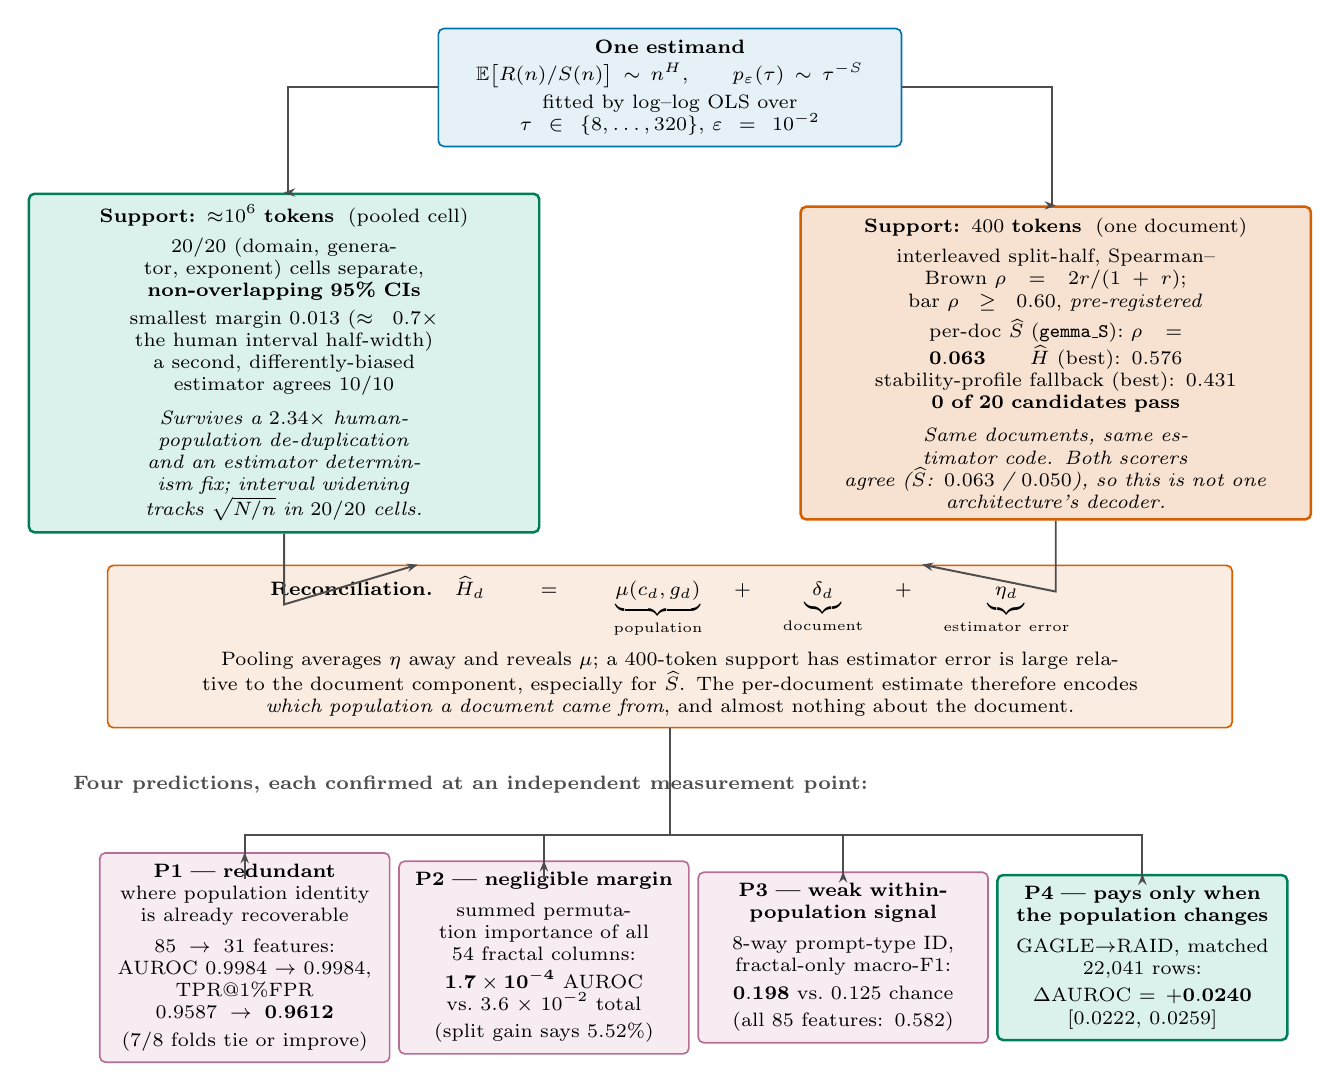
\begin{tikzpicture}[x=1cm,y=1cm,font=\scriptsize]

% ------------------------------------------------------------- the estimand
\node[phase, minimum width=48mm, text width=56mm] (est) at (8.0,7.1)
  {\textbf{One estimand}\\[2pt]
   $\mathbb{E}\big[R(n)/S(n)\big]\sim n^{H}$,\qquad
   $p_{\varepsilon}(\tau)\sim\tau^{-S}$\\[2pt]
   fitted by log--log OLS over $\tau\in\{8,\dots,320\}$, $\varepsilon=10^{-2}$};

% --------------------------------------------------------------- left: pooled
\node[passnode, minimum width=54mm, text width=62mm] (pool) at (3.1,3.6)
  {\textbf{Support: ${\approx}10^{6}$ tokens} \;(pooled cell)\\[3pt]
   $20/20$ (domain, generator, exponent) cells separate,\\
   \textbf{non-overlapping 95\% CIs}\\[2pt]
   smallest margin $0.013$ ($\approx0.7\times$ the human interval half-width)\\
   a second, differently-biased estimator agrees $10/10$\\[4pt]
   \emph{Survives a $2.34\times$ human-population de-duplication}\\
   \emph{and an estimator determinism fix; interval widening}\\
   \emph{tracks $\sqrt{N/n}$ in $20/20$ cells.}};

% ------------------------------------------------------------ right: per-doc
\node[failnode, minimum width=54mm, text width=62mm] (doc) at (12.9,3.6)
  {\textbf{Support: $400$ tokens} \;(one document)\\[3pt]
   interleaved split-half, Spearman--Brown $\rho=2r/(1+r)$;\\
   bar $\rho\ge0.60$, \emph{pre-registered}\\[2pt]
   per-doc $\widehat S$ (\texttt{gemma\_S}): $\rho=\mathbf{0.063}$\qquad
   $\widehat H$ (best): $0.576$\\
   stability-profile fallback (best): $0.431$\\
   \textbf{0 of 20 candidates pass}\\[4pt]
   \emph{Same documents, same estimator code. Both scorers}\\
   \emph{agree ($\widehat S$: $0.063$ / $0.050$), so this is not one}\\
   \emph{architecture's decoder.}};

\draw[flow] (est.west) -- ++(-1.9,0) |- (pool.north);
\draw[flow] (est.east) -- ++( 1.9,0) |- (doc.north);

% -------------------------------------------------------------- the mechanism
\node[finding, minimum width=126mm, text width=140mm] (mech) at (8.0,0.0)
  {\textbf{Reconciliation.}\quad
   $\widehat H_d \;=\; \underbrace{\mu(c_d,g_d)}_{\text{population}}
                 \;+\; \underbrace{\delta_d}_{\text{document}}
                 \;+\; \underbrace{\eta_d}_{\text{estimator error}}$\\[4pt]
   Pooling averages $\eta$ away and reveals $\mu$; a $400$-token support has
   estimator error is large relative to the document component, especially for
   $\widehat S$. The per-document
   estimate therefore encodes\\ \emph{which population a document came from},
   and almost nothing about the document.};

\draw[flow] (pool.south) -- ++(0,-0.9) -- ($(mech.north)+(-3.2,0)$);
\draw[flow] (doc.south)  -- ++(0,-0.9) -- ($(mech.north)+( 3.2,0)$);

% ------------------------------------------------------------- four predictions
\node[grouplab, anchor=west] at (0.3,-1.75)
  {Four predictions, each confirmed at an independent measurement point:};

\node[evalnode, minimum width=30mm, text width=34mm] (p1) at (2.6,-3.95)
  {\textbf{P1 --- redundant}\\ where population identity is already
   recoverable\\[3pt]
   $85\to31$ features:\\ AUROC $0.9984\to0.9984$,\\
   TPR@1\%FPR $0.9587\to\mathbf{0.9612}$\\[2pt] ($7/8$ folds tie or improve)};

\node[evalnode, minimum width=30mm, text width=34mm] (p2) at (6.4,-3.95)
  {\textbf{P2 --- negligible margin}\\[3pt]
   summed permutation importance of all 54 fractal columns:\\[2pt]
   $\mathbf{1.7\times10^{-4}}$ AUROC\\ vs.\ $3.6\times10^{-2}$ total\\[2pt]
   (split gain says $5.52\%$)};

\node[evalnode, minimum width=30mm, text width=34mm] (p3) at (10.2,-3.95)
  {\textbf{P3 --- weak within-population signal}\\[3pt]
   8-way prompt-type ID,\\ fractal-only macro-F1:\\[2pt]
   $\mathbf{0.198}$ vs.\ $0.125$ chance\\[2pt] (all 85 features: $0.582$)};

\node[passnode, minimum width=30mm, text width=34mm] (p4) at (14.0,-3.95)
  {\textbf{P4 --- pays only when the population changes}\\[3pt]
   GAGLE$\to$RAID, matched\\ $22{,}041$ rows:\\[2pt]
   $\Delta$AUROC $=\mathbf{+0.0240}$\\ $[0.0222,\,0.0259]$};

\foreach \n/\x in {p1/2.6, p2/6.4, p3/10.2, p4/14.0}{
  \draw[flow] ($(mech.south)+(0,0)$) -- ++(0,-1.35) -| (\x,-2.95) -- (\n.north);
}

\end{tikzpicture}
}
\caption{One estimand, two supports. \emph{Left:} pooled, the exponents
separate in $20/20$ cells with non-overlapping intervals. \emph{Centre:} the
same documents at $400$-token support give $\rho=0.063$ for \Sest\ and $0/20$
features clearing $\rho\ge0.60$. \emph{Right:} the four predictions
Eq.~\ref{eq:decomp} makes, each confirmed independently.}
\label{fig:dissociation}
\end{figure}

All measurements are on GAGLE \citep{alabdulmohsin2025tale}: five domains $\times$
two generators (Gemma-2B, Mistral-7B) $\times$ three temperatures $\times$ eight
prompt types, plus the human source articles. After the token-window gate the store
holds $223{,}834$ documents --- $112{,}402$ Gemma-2B, $106{,}432$ Mistral-7B,
$5{,}000$ human --- at a human prevalence of $2.234\%$. Each carries $85$ features
in three families, enumerated in full in Appendix~\ref{app:features}: \textbf{A
(fractal, $54$)}, both exponents with fit quality, uncertainty, per-scale residuals
and windowed profiles; \textbf{B (token-statistical, $17$)}, log-perplexity moments,
rank buckets \citep{gehrmann2019gltr} and entropy; \textbf{C (discourse/style,
$14$)}, length, repetition and dispersion statistics on a ratio-derived word budget
so they cannot degenerate into length proxies. Family-B features are written only
above an $r_{\text{align}}\!\ge\!0.98$ gate, GAGLE's precomputed scores recording neither
checkpoint nor tokenizer.
% source: findings/results/p3_tables.md; writing/methodology.md S2; docs/OVERVIEW.md S3

\subsection{Q1: the ensemble gap survives full re-derivation}
\label{sec:ensemble_gap}

Before treating the corpus-level separation as established, we audited it
against two potential confounds in the corpus and estimator pipeline, and
report the fully audited result below rather than the first version measured.
% source: reports/2026-08-24_X02_aggregate_fractal_gap_survives.md
First, population: GAGLE's split label was treated as part of an article's
identity, so the same article recurred as several ``different'' human
documents; collapsing these duplicates takes the human $N$ from
$\approx11{,}700$ to $5{,}000$. Second, estimator determinism: the H\"older
estimator sampled window starts rather than enumerating them, so every stored
per-document \Sest\ carried Monte-Carlo noise; enumerating them removes it.
Both audits are resolved, and every $S$-based interval below is recomputed
on one estimator vintage; the smallest margin anywhere is \texttt{wikipedia}
\Strue\ under Gemma-2B, a gap of $0.013$, about $0.7$ of the human interval's
half-width (Table~\ref{tab:x02}, Appendix~\ref{app:corpuschecks}). \textbf{A second,
differently biased estimator agrees}: bootstrapping the mean of per-document
point estimates separates every cell in the same direction, $10/10$ on
\Strue\ (two further checks and a replication note: Appendix~\ref{app:corpuschecks}).

\subsection{Q2: the pre-registered reliability gate, and its failure}
\label{sec:reliability}

The check was specified, with its threshold, before any detection experiment was
run. Each document's token sequence is split into \emph{interleaved} odd/even
halves --- not first-half/second-half, which would confound estimator unreliability
with genuine stylistic drift between a document's opening and its close --- both
exponents are refit independently on each half, and the half-length correlation is
Spearman--Brown corrected, $\rho = 2r/(1+r)$, against a $\rho\ge0.60$ bar declared
in advance.

\paragraph{The interleaving assumption, and its scope.} Both estimators are
functionals of sequential geometry, so it is fair to ask whether decimating
the sequence changes the object measured. Under this paper's own premise it
does not: for a process exactly self-similar with stationary increments ---
the premise that makes $\Htrue$ and $\Strue$ well defined at all --- decimation
by two \emph{is} the dilation the scaling law is invariant under, so each half
carries the same exponent up to a known constant. \textbf{What the objection
does reach is the gap between exact scaling and real text}, outside that
argument, so we tested the sensitivity of $\rho$ to the split construction
directly rather than leaving it open.
% source: reports/2026-08-23_P2_split_half_reliability.md; review_results/data/t0_t1_MERGED_table.json

\paragraph{The split-construction test.} Eight constructions were run end to
end on the full corpus (enumerated, with a ninth measured but excluded as
invalid, in Appendix~\ref{app:reliability}).
\textbf{Reliability declines smoothly and monotonically as the block grows}
--- \texttt{gemma\_H}: $0.576\to0.562\to0.549\to0.534\to0.501$ for block sizes
$1,4,8,16,32$ --- the opposite of what the sequence-geometry objection
predicts: if decimation damaged the estimand, coarser blocks should
\emph{recover} reliability, and instead single-token interleaving is the
best-performing of the eight, tied by the full sweep. Only \texttt{contiguous} falls
outside the band every other construction shares, the pre-registered,
\emph{expected} signature of the drift confound the design exists to avoid.
\textbf{Interleaving is not the outlier that inflates $\rho$; it is the
construction that damages the sequence least.}

\textbf{Zero of twenty candidates pass}, and the result separates into two
qualitatively different findings (full table, Appendix~\ref{app:reliability}).
\Hest\ has modest but genuine reliability falling just short of the bar
($\rho=0.576$ for \texttt{gemma\_H}, $0.547$ for \texttt{mistral\_H}); \Sest\ has
essentially none ($0.063$ and $0.050$). \textbf{Read $\rho=0.063$ concretely:
at $N\!\approx\!400$ tokens (a few short paragraphs), measure one document's
H\"older exponent on its odd tokens and again on its even tokens, and the two
answers agree about as well as two documents chosen at random.} That is not a weak effect: no plausible
correction moves $0.06$ to $0.60$, and the natural rescue fails with it --- the
pre-registered windowed-stability fallback tops out at $0.431$ and bottoms out
at $0.003$, a shorter instrument rather than more curve
(Appendix~\ref{app:reliability}). \textbf{The two exponents fail differently
and we do not treat them as one:} \Sest\ is unreliable here, while \Hest\ is
moderately reliable and below the bar by more than sampling error --- at
$n=221{,}904$ its Fisher-$z$ $95\%$ interval is $[0.573,0.580]$, so \Hest\ misses
by construction, not by noise. The result is architecture-independent across a
$2$B Gemma and a $7$B Mistral, taken \emph{after} the estimator's earlier
non-determinism was fixed and the corpus regenerated.

\paragraph{Estimator ablation: DFA and local Whittle.} \textbf{The verdict is
mixed and we report it as mixed.} Refit on the identical halves, local
Whittle clears the bar for both scorers ($\rho=0.677$/$0.642$); DFA clears it
for Gemma only, marginally, and misses for Mistral. R/S and DFA correlate at
$0.87$/$0.86$ (the same exponent, less noisily estimated); R/S and Whittle
correlate at only $0.76$/$0.75$, so part of Whittle's headroom is not shared
with the exponent \Hest\ is defined against (full numbers and a third,
geometric estimator: Appendix~\ref{app:reliability}). \textbf{Neither estimator touches
\Sest}, whose reliability stands exactly where \S\ref{sec:reliability}
already put it.
% source: review_results/data/t4_alt_estimators_reliability.json

\paragraph{Estimator bias against ground truth, by support.} Reliability and
bias are separate properties and this estimator is compromised on both:
validated against synthetic fractional Brownian motion of known exponent, at
document support \Sest\ is biased $-0.26$ to $-0.48$, and more bootstrap
draws at the same fixed support do not close the gap (full ladder and
pooling-mode bias: Appendix~\ref{app:reliability}). Since every machine cell
sits above its matched human cell in the pooling mode actually used, this
bias is conservative for the ensemble gap: understated, not manufactured.
% source: reports/2026-07-26_S_estimator_fix.md

\paragraph{Reliability as a function of support, and where it crosses the bar.}
The bound above says how much of $\rho_{\text{pooled}}$ is population; it does
not say how much \emph{support} would fix the rest. We calibrate an estimator
noise floor against synthetic fractional Gaussian noise at GAGLE's own observed
$\Htrue\in[0.60,0.72]$ band and compose $\rho_{\text{SB}}(N)=2r(N)/(1+r(N))$
across $N\in\{100,\ldots,12{,}800\}$ (Figure~\ref{fig:nstar},
Appendix~\ref{app:reliability}). \Hest\ crosses the bar at $N^{\star}=800$ ---
already $\rho_{\text{SB}}=0.49$/$0.46$ at $N=400$, close to GAGLE's own support
--- while \Sest\ needs $N^{\star}\!\ge\!6{,}400$, sixteen times what any
document here supplies. A companion pass over $5{,}000$ full-length human
documents confirms the floor is not an underestimate of real-text scatter
(median full-document $\Hest=0.629$, inside the band). \textbf{That check is
\Hest-only}: for \Sest\ it predicts $0.229$/$0.197$ at $N=400$ against
$0.063$/$0.050$ measured, so \Sest's $N^{\star}$ is a \emph{lower} bound.
\textbf{The asymmetry between the two
exponents is now quantitative, not just qualitative}: \Hest's shortfall
resolves at roughly twice GAGLE's token budget; \Sest's does not resolve
within an order of magnitude of it.
% source: review_results/data/t2_n_star_composition.json; review_results/FINDINGS_LEDGER.md T2

The gate's designed output, a whitelist of surviving fractal features, was
emitted empty; the detection stage trains on all $54$ from a manifest declared
in advance instead, the bar stays at $0.60$, and the features are carried
forward so the ablation below can price them independently.
% source: writing/methodology.md S3

% =============================================================================
\section{What the Document-Level Estimate Represents}
\label{sec:consequences}

That the per-document estimate is dominated by estimator error at this
support is a statement about an instrument, and on its own proves nothing
about detection --- an unreliable quantity could still be useful by
accident. This section and the two that follow run the four tests of
Table~\ref{tab:map} in the order \S\ref{sec:analogy} laid out: P1 and P2
first, as necessary conditions a rival explanation could also satisfy; P3
next, as the critical test only this account survives; P4 last, as the
falsification control.

\paragraph{The instrument.}
The learner is deliberately unremarkable and held fixed across every
comparison: a class-weighted gradient-boosted tree ensemble, splits frozen
before training and group-disjoint by seed article. Eight folds cross five
confound configurations, arms and learners ($304$ cells,
$2{,}000$-fold bootstrap intervals);
the headline metric is recall at fixed low FPR, not AUROC. Two controls are
load-bearing (Appendix~\ref{app:detection}): a label-shuffle harness landing
systematically \emph{below} chance, and an explicit pricing of the length
confound, a two-feature \arm{length\_only} arm reaching AUROC $0.8635$ at
TPR@$1\%$FPR $0.0477$.
% source: writing/methodology.md S4; findings/results/p3_tables.md RANDOM config 1

\subsection{P1 and P2 --- Necessary Conditions: Redundant In-Distribution, Worthless at the Margin}
\label{sec:p1}

\emph{In the story: a second thermometer, handed to someone who already knows which
country they are standing in.} Deleting all $54$ features leaves AUROC unchanged to four decimals
and \emph{improves} recall at $1\%$ FPR from $0.9587$ to $0.9612$: a
$31$-feature model matches an $85$-feature one (full arm grid,
Appendix~\ref{app:detection}). \textbf{This outcome is predicted by
\S\ref{sec:reliability}, not merely consistent with it.} Without the
reliability measurement in hand, a family separating human from machine text
in $20$ of $20$ cells yet contributing nothing to a classifier on the same
corpus reads as a modelling failure and invites an architecture search. It is
neither: $\rho=0.063$ says the estimate is a population-conditional mean plus
noise, and perplexity and style already identify the population, so the
fractal columns arrive carrying information the model has, wrapped in
variance it does not want. A fractal-only model reaches AUROC $0.6629$ above
chance, but the family is neither necessary nor additive: \arm{fractal+stat}
sits \emph{below} \arm{stat\_only}, \arm{all\_minus\_fractal} ties or wins on
$7$ of $8$ frozen folds, and a shallow MLP reproduces the pattern
(Appendix~\ref{app:detection}).

P2 is the fingerprint. Split gain over all $85$ inputs credits the $54$
fractal columns with $5.52\%$ of the total, and the model splits on every one
at least $125$ times. Permutation importance on the held-out fold tells the
opposite story: the summed AUROC drop across all $54$ is
$\mathbf{1.7\times10^{-4}}$ against $1.54\times10^{-2}$ and $2.04\times10^{-2}$
for the other two families --- $0.47\%$ of the total against a $5.52\%$ gain
share, with $35$ of $54$ zero or negative (full breakdown,
Appendix~\ref{app:importance}). \textbf{Used constantly, worth nothing.}
% source: findings/results/p3_tables.md, "Feature importance -- ALL declared features (D-13)"

\subsection{P3 --- The Critical Test: Eliminating the Last Alternative Explanation}
\label{sec:withinpop}

\emph{In the story: two houses on the same street.} P1 and P2 show the
representation is redundant and marginally worthless; neither shows
\emph{why}, since both are measured where the population term is available.
Eight-way prompt-type identification, run on machine-generated GAGLE rows
only, removes that escape route: GAGLE is a complete $240$-cell factorial
($2$ generators $\times\,3$ temperatures $\times\,5$ domains $\times\,8$
prompt types), so prompt type is crossed with every population factor
\emph{by the corpus's own design}. \textbf{$\mu$ varies across documents but
is balanced across the labels being separated}, contributing variance
without contributing signal --- \emph{of the tests here, this is the one
best placed to have falsified the account.}
% source: data/p5_task3_prompt_type_id.json
\textbf{The task is solvable, and the fractal representation recovers little of
it.} Chance is macro-F1 $0.125$. All $85$ features reach $0.5816$
\ci{0.5747}{0.5885}, so these eight classes genuinely differ document by
document; the $54$ fractal features alone reach $0.1981$ \ci{0.1919}{0.2043}
--- \textbf{about a sixth of the distance} from guessing to what the corpus
supports, from a family with $1.7\times$ as many columns as the incumbents.
\textbf{We do not stop at asserting the balance survives the gates; we
measured it}, with three checks that close the residual-confound route
directly (full numbers, Table~\ref{tab:withinpop}, Appendix~\ref{app:withinpop}):
a population-only control (generator, domain, temperature, no prompt type)
scores \emph{below} chance ($0.0594$, floor $0.125$); the factorial survives
the token-window and complete-case gates with a maximum cell deviation of
$0.22$ percentage points; and removing each fractal column's stratum mean
% AUDIT FIX: 0.2046 lies just outside the 0.1981 interval [0.1919,0.2043], so
% "within its confidence interval" is false; adopted Appendix H's own correct
% phrasing ("confidence intervals overlapping", Table \ref{tab:withinpop}).
before refitting leaves fractal-only macro-F1 \emph{unchanged, its confidence
interval overlapping} ($0.1981\to0.2046$) rather than falling toward chance.
\textbf{Together these rule out the residual-population-confound explanation
rather than merely bound it}: the signal is genuine document-level structure,
not population leakage. This is a within-population discriminative test, not a
direct estimate of $\mathrm{Var}(\delta)$, and does not reference the
split-half gate --- so $\rho=0.063$ should be read as a property of the
estimand--support relationship, not an artifact of how we split tokens. The
number most exposed by this analysis is unchanged: $0.5816$, not $0.1981$.
% source: review_results/data/t3_population_control.json; review_results/FINDINGS_LEDGER.md T3

Two further within-corpus results separate the same two terms (full folds and
numbers: Appendix~\ref{app:detection}). \emph{Substitution}, a question about
$\delta$: the fractal arm loses on \textbf{all eight of eight} folds against
\arm{stat\_only}. \emph{Generator identity}, a question about $\mu$, is easy
by contrast: AUROC $0.9943$, same corpus, same features. \textbf{Same
features, same corpus, same classifier: near-chance when asked about the
document, near-perfect when asked about the population.} Where the detector
actually fails is not a fractal story either --- a tail-ranking failure on
\texttt{billsum} LODO driven by prompt type, whose largest shifts are style
features.
% source: findings/results/p0_p5_audit.md S3.3; data/p5_task2_gagle_generator_id.json

% =============================================================================
\section{The Structural Probe: Direct Evidence for the Mechanism}
\label{sec:perturb}

\emph{In the story: jostling the thermometer while you read it, versus
repainting the house it stands in.} \textbf{This section is a targeted
diagnostic of what the fractal features are keyed to, not an
adversarial-robustness benchmark; its Class I result is the paper's
strongest evidence for the proposed mechanism.} We ask what structure the
representation reads, not how much recall an attack removes, using two kinds
of edit that destroy different things. The scaling estimators of
\S\ref{sec:background} are functionals of one structure only, the ordered
token index: indifferent to \emph{which} words appear, sensitive only to
their arrival order. The bank splits on that axis: \textbf{Class I (order)}
--- \texttt{sentence\_reorder}, \texttt{typo\_noise} --- scrambles
\emph{where} tokens sit, not \emph{which} words they are; \textbf{Class II
(content)} --- four paraphrase/style/summarize operators --- swaps
\emph{which} words appear at fixed coarse-scale order
(Appendix~\ref{app:battery}). A document-level property should need Class I
most; population identity plus estimator noise should make Class I actively
\emph{harmful} instead.

The battery applies six operators to GAGLE machine text, yielding $39{,}810$
(document, variant) pairs, each passing a semantic-preservation guard (full
grid, detector list and definitions: Appendix~\ref{app:battery}). The tabular
detector (Table~\ref{tab:attackablation}) stays above $0.92$ on every Class
II operator and collapses to $0.2670$ on \texttt{sentence\_reorder}, while
Binoculars \citep{hans2024binoculars} degrades roughly uniformly and a
fine-tuned RoBERTa is unmoved.
% source: writing/methodology.md S5; findings/results/p4_robustness.md

Retraining the fractal-free $31$-feature model on the same edited population,
the partition predicts the sign in six of six cases: full model ahead by
$0.94$--$2.10$ points on all four Class II operators, and \emph{deleting} the
fractal family \emph{raises} recall by $1.96$ and $8.76$ points on
\texttt{sentence\_reorder}/\texttt{typo\_noise} --- once order is scrambled,
fractal features vote against the right answer, and dropping them recovers
it.
% source: reports/2026-08-30_fractalscope_verification_checks.md S1, S3

\textbf{This Class I reversal is why this section is diagnostic, not a
secondary robustness check.}
\texttt{sentence\_reorder} and \texttt{typo\_noise} are the only two operators
that attack the \emph{support} rather than the \emph{content}, preserving the
lexical statistics every other feature reads and perturbing only the index
Family A claims to measure. A representation that genuinely encoded that
structure would degrade under them; instead the contribution \emph{flips
sign} precisely and only here. \textbf{A feature family cannot be a
measurement of sequence structure and also be actively harmful when, and only
when, sequence structure is perturbed.} This is what
$\mathrm{Var}(\eta)\gg\mathrm{Var}(\delta)$ predicts, and it isolates $\delta$
without relying on the split-half gate (mechanism and qualifications:
Appendix~\ref{app:battery}).

% =============================================================================
\section{P4 --- Where Ensemble Structure Does Transfer, and Why That Is Not a Rebuttal}
\label{sec:transfer}

\emph{In the story: you move to a different country, and the same $\pm5^\circ$
thermometer starts telling you something again.} \textbf{This subsection
addresses the one result that, at first reading, appears to contradict the
paper's central claim.} Three sections have just shown a feature family to be
redundant, marginally worthless and near-chance within a population; here the
same family buys a statistically significant $+0.0240$ AUROC. If that were
evidence the features carry document information after all, the argument
would collapse. It is not, and the reason is the thermometer that has not
changed while the climate around it has.

We test P4 on RAID \citep{dugan2024raid}, $11$ generators and $8$ domains
re-scored through the identical pipeline and used only as an external test,
with \emph{no} retraining. Crossing corpora costs $0.195$ AUROC
($0.9984\!\to\!0.8032$) and $0.731$ recall at $1\%$ FPR
($0.9587\!\to\!0.2277$) --- the largest degradation anywhere in this
evaluation --- and the fractal family's advantage survives on a
composition-matched population (Table~\ref{tab:raid}, Appendix~\ref{app:multiclass}):
small, $+0.0240$ AUROC on a model that is itself badly degraded, and real.
% source: feature_store/v3_raid.parquet 68,212 x 90;
%         data/p5_task4_gagle_to_raid_transfer.json;
%         reports/2026-08-30_fractalscope_verification_checks.md S4

\subsection*{Testing the population-mean explanation directly}

\textbf{What moved is $\mu$; $\delta$ is as absent here as in
\S\ref{sec:withinpop}.} Crossing to RAID changes the populations, and the
fractal columns --- carrying a coarse population mean that still correlates
with generator identity in the new corpus --- are left holding the one thing
that survived. Tested directly: \textbf{replacing} each document's $54$
fractal columns with its $(\text{generator},\text{domain})$ group mean
\emph{recovers more than the entire} gap (AUROC $0.8149$, $149\%$ of it), and
\textbf{subtracting} it retains $59\%$ (AUROC $0.7934$) --- population
information does the majority of the work, with a real document-level
residual (full arms, Appendix~\ref{app:multiclass}). \textbf{The honest
reading is not ``fractal features are robust'' but ``the ensemble term is the
part that travels'', now shown rather than only argued.}
% source: review_results/data/t5_raid_group_mean.json

\textbf{What would have to be true for this to be a rebuttal is not true.} A
document-level source for the $+0.0240$ would require these features to
carry document-level content somewhere; on the one task holding the
population fixed they reach $0.198$ against a $0.125$ floor. Three facts
bound it the same way: the gain appears only after the model has already
lost $0.195$ AUROC crossing corpora; \arm{fractal\_only} does not transfer;
and it is population-level by construction, generator identity within GAGLE
being recoverable at AUROC $0.9943$ from features that cannot separate two
machine-written articles. \textbf{Read as a recommendation, P4 says keep
these columns when you expect the population to change, and never expect
them to describe the document in front of you.} This is a
\emph{complete-case} result covering $32\%$ of RAID's rows (excluded
majority: Appendix~\ref{app:limitations}).

\section{A Second Measurement Illusion: Scorer--Attacker Lineage Inflates Measured Robustness}
\label{sec:lineage}

\textbf{This section is methodologically independent of everything
above} --- it uses the same edit battery but is not about fractal features,
and nothing in \S\ref{sec:ensemble}--\S\ref{sec:transfer} depends on its
result, nor does it depend on theirs. What it shares with them is the
paper's actual thesis: a measurement can look like it is reading the
document in front of it while it is really reading an artifact of how the
evaluation was built. There, the artifact was population identity smuggled
in as document content; here, it is the attacker model's kinship with the
scorer smuggled in as robustness. We give it its own section, with its own
evidence, rather than folding it into the fractal argument, because it is
reproducible on its own, requires none of that argument's machinery to
check, and will silently affect any robustness evaluation built the way
ours was.

\textbf{Fast-DetectGPT's recall \emph{rises} under every Class II operator}, from a
$0.5104$ baseline to $0.63$--$0.86$ --- at face value, paraphrasing making machine
text easier to detect, the opposite of this literature's central finding
\citep{krishna2023paraphrasing,sadasivan2023canai}. It is neither a floor artifact
(far above our $15\%$ no-signal screen) nor robustness: Fast-DetectGPT
scores curvature under Gemma-2B, and these paraphrases were generated by a model in
Gemma's own lineage, so the edited text is maximally predictable \emph{to the
scorer} and the attack raises the detector's key signal instead of defeating it.
Regenerating the same paraphrase outside that lineage collapses recall to
$1.2$--$4.5\%$ across a capability ladder of five external models on
$5{,}000$ documents, and the reversal is stable, the tabular detector
degrading broadly monotonically with attacker size ($72.6\%\!\to\!36.5\%$)
and Binoculars tracing the cleanest curve ($70.8\%\!\to\!35.1\%$;
Appendix~\ref{app:ladder}). \textbf{Scorer--attacker lineage, not detector
design, determines whether a curvature-based detector appears robust to
paraphrase.} \textbf{The check is cheap: regenerate one attack type with a
model outside the scorer's lineage and compare.}
% source: findings/results/p4_robustness.md S3

% =============================================================================
\section{Discussion, Limitations, and Conclusion}
\label{sec:limitations}

\paragraph{A claim about measurement, not about the existence of fractal structure.}
Nothing here contradicts language's fractal information structure, or model
output's departure from it. This paper adds the second half: an exponent
defined by an asymptotic law, estimated on a $400$-token realisation across
$1.6$ decades, resolves the process far better than the realisation, and the
whole curve does not rescue it. Support from outside this estimator family:
\citet{wei2025shortphd} find a topological scaling dimension on
\emph{embeddings} degrading at short length for the same reason, and
\citet{yang2026turbulence} report a $5/3$ spectrum disrupted by
randomization of token order. \textbf{We also tested this directly} on a
representation with no fractal machinery at all --- overlapping-window
MiniLM embeddings reduced to persistent-homology loop statistics, at zero
content overlap between halves: no window geometry tried clears \Hest's own
reliability (best genuine value $0.41$; full pilot,
Appendix~\ref{app:limitations}), evidence for the generality of the
mechanism, not only for this estimator family.
% source: review_results/data/t10_pilot_geometry_comparison.json; review_results/FINDINGS_LEDGER.md T10

For deployment the reading is regime-dependent: drop the family within a
known corpus (redundant at best, costing $8.76$ points of recall at worst);
keep it for a detector that must generalise ($+0.0240$ AUROC).
\textbf{No detector evaluated here supports consequential accusations
against individuals}: the best loses $73$ points of recall crossing corpora.

\paragraph{Limitations.}
Appendix~\ref{app:limitations} states each with its numbers, and one is a
contribution in its own right: \emph{perturbation-response fusion requires a
class-symmetric edit battery}, since on a $9{,}997$-of-$9{,}997$
machine-generated population a drift feature exists only for the positive
class, and a classifier given it learns population membership rather than
robustness. The sensitivity of $\rho$ to the split construction and the
token support at which it clears the bar, previously open, are now measured
(\S\ref{sec:reliability}); matched-length bands, RAID complete-case
composition, deployment-prevalence recalibration and a second representation
family are in Appendix~\ref{app:limitations}. Beyond these: no architectural
account of the exponents; no coverage of human revision; a single scorer
pair, one corpus family, English only; an uncorrected $65$-comparison run;
and two feature-extraction defects found during review, after which every
store was rebuilt, every number post-correction \emph{with one marked
exception} (Table~\ref{tab:attackablation}).
% source: reports/2026-08-30_fractalscope_verification_checks.md S5

\paragraph{Conclusion.}
The fractal signature of machine-generated text is real, and at this support
it is not a document representation: $20$ of $20$ cells separate in
ensemble, $0$ of $20$ split-half candidates clear a pre-registered bar at
$400$ tokens, and all four predictions of Table~\ref{tab:map} hold. We
propose as a measurement-validity criterion, not a theorem: a scaling
statistic should not be read as a stable document-level measurement without
a reliability coefficient at the support on which it is used.

\subsection*{AI use statement}

In this work, we used generative AI tools for none of the tasks carrying a
required disclosure: no part of the research ideation, hypothesis formulation,
experimental design, theoretical framework, or interpretation of results was
generated by an AI system, no synthetic data sets were produced by generative AI
for use as evidence, and no mathematical or empirical claim originates from an
AI system. Generative AI was used for tasks in the recommended-disclosure
category only: drafting and copy-editing prose in this manuscript, literature
search and retrieval of candidate related work, and assistance with LaTeX
formatting and figure code. Every AI-assisted passage was checked against the
underlying artifact it describes --- each numeric claim in this paper carries a
source comment in the LaTeX naming the file it was read from, and those were
verified by the authors against the artifacts on disk rather than accepted from
a generated draft. All retrieved references were opened and their venue, author
list and content confirmed by the authors before citation. We take
responsibility for the final content of this work, including all text, claims
and artifacts.

\subsection*{Ethics statement}

Detection of machine-generated text is dual-use, and this paper's structural
analysis is more dual-use than a detector would be: the operator partition of
\S\ref{sec:perturb} tells a defender which feature family to drop and tells an
attacker which edit class to prefer. We judge publication net positive on three
grounds. First, the vulnerability reported --- a published feature family
degrading under sentence reordering and character noise --- concerns an existing,
already-public construction rather than a novel attack technique, and both
operators are trivially available. Second, the paper's operational
recommendation is simplification, dropping a costly and unreliable component,
not disclosure of an exploit. Third, the scorer--lineage finding
(\S\ref{sec:lineage}) corrects an evaluation error that currently causes
robustness to be \emph{overstated}, which is a defender-side benefit. Against
that: false accusation is the dominant harm in the settings where these systems
are used, which is why every headline number here is recall at $1\%$ or $5\%$
false-positive rate rather than AUROC, and why \S\ref{sec:limitations} states
plainly that no detector evaluated here supports consequential individual
accusations. We did not measure per-writer-population false-positive rates --- in
particular for non-native writers, where detector bias is documented --- and we
flag that absence rather than let low aggregate FPR imply low FPR for every
group. All data are existing public research corpora (GAGLE, RAID); no new
human-subjects data was collected, and no human annotation was commissioned.

\subsection*{Reproducibility statement}

Every number in this paper is reproducible from artifacts already on disk
without re-running any generation or scoring pass. Splits are frozen and
versioned (\texttt{data/splits\_v1.json}) and reused unchanged by the robustness
and transfer stages, which is what makes their numbers comparable to the
detection stage's. Metric implementations are frozen in a single
\texttt{eval/metrics.py}; all intervals are $95\%$ percentile bootstrap at
$2{,}000$ resamples, stratified by class for binary metrics, and intervals
resting on fewer than $2{,}000$ usable resamples are marked as such. The $54$
fractal features are declared in advance in
\texttt{feature\_store/p3\_feature\_manifest.json}; the reliability gate's
output, including its empty whitelist and twenty rejected entries, is in
\texttt{feature\_store/p2\_reliability\_report.json}. The training pipeline
(class weighting, prefit sigmoid calibration on the validation fold, threshold
derivation from the validation ROC) is implemented once and reused without
modification by every downstream script. The one arm not in the original grid ---
\arm{all\_minus\_fractal} scored against the edit battery and RAID --- was
retrained through that same pipeline and confirmed to reproduce the frozen
in-distribution AUROC to five decimals before any number from it was used.
\textbf{One artifact we audited and could not clear}: the $85$-feature model's
operating-threshold file has four consumers and no writer in the repository, and
re-deriving the $1\%$ and $5\%$ FPR thresholds from the frozen model across
$\{$calibrated probability, raw probability, raw margin$\}\times\{$validation,
test$\}$ reproduces \emph{none} of the stored values, with a gap that is not a
rounding miss ($6\!\times\!10^{-4}$ on the $1\%$ threshold $t_{1}$,
$1.7\!\times\!10^{-2}$ on the $5\%$ threshold $t_{5}$). The full audit, including the $5\%$ threshold's staleness and the $1\%$
threshold's internal inconsistency, is in Appendix~\ref{app:thresholds}; the
consequence for this paper is bounded and marked where it bites.

% =============================================================================
\bibliographystyle{iclr2027_conference}
% AUDIT FIX: bibliography filename did not match the .bib shipped in this directory (references_090926.bib); all 33 citations compiled as undefined.
\bibliography{references_090926}

% =============================================================================
% =============================================================================
\appendix

\section{Corpus-Level Gap: Supporting Checks}
\label{app:corpuschecks}

\begin{table}[h]
\centering
\caption{Corpus-level pooled exponents after both corrections; $95\%$ intervals,
$10$-fold outer bootstrap re-pooling raw trajectories. Human $n=1{,}000$ per domain,
machine $n\approx21{,}000$--$22{,}700$ per cell, all scored under Gemma-2B. No
interval overlaps its domain's human interval on either exponent for either
generator: $20/20$. Source: \texttt{data/x02\_confidence\_intervals.json}.}
\label{tab:x02}
\scriptsize
\setlength{\tabcolsep}{3.4pt}
\begin{tabular}{lccc@{\hskip 5mm}ccc}
\toprule
& \multicolumn{3}{c}{\textbf{H\"older \Strue}} & \multicolumn{3}{c}{\textbf{Hurst \Htrue}}\\
\cmidrule(lr){2-4}\cmidrule(lr){5-7}
Domain & Human & \texttt{gemma\_2b} & \texttt{mistral\_7b}
       & Human & \texttt{gemma\_2b} & \texttt{mistral\_7b}\\
\midrule
\texttt{big\_patent}       & [.4135,.4283] & [.4762,.4806] & [.4929,.5012] & [.6365,.6415] & [.6891,.6911] & [.7123,.7141]\\
\texttt{billsum}           & [.3992,.4268] & [.4541,.4638] & [.4478,.4538] & [.6315,.6368] & [.6674,.6693] & [.6859,.6879]\\
\texttt{newsroom}          & [.3539,.3794] & [.4627,.4668] & [.4888,.4917] & [.6021,.6122] & [.6613,.6635] & [.6893,.6918]\\
\texttt{scientific\_papers}& [.3896,.4046] & [.4659,.4719] & [.4965,.5037] & [.6068,.6118] & [.6864,.6889] & [.7131,.7156]\\
\texttt{wikipedia}         & [.3944,.4301] & [.4428,.4505] & [.4657,.4705] & [.6208,.6279] & [.6550,.6569] & [.6754,.6773]\\
\bottomrule
\end{tabular}
\end{table}


Two further checks on \S\ref{sec:ensemble_gap}'s $20/20$ separation, plus a
replication failure on the source publication's separate \emph{spread} claim.

The duplicate-count finding itself: GAGLE's split label had been treated as part of an
article's identity, so the same article recurred as several ``different''
human documents. Every one of the $4{,}474$ cross-split copies checked is
byte-identical, and collapsing all duplicate groups takes the human population
from $\approx11{,}700$ rows to $5{,}000$ articles, a $2.34\times$ over-count.
The $4{,}474$ is the byte-identity verification count, not the number of rows
removed; the reduction itself is the $\approx6{,}700$ excess copies.

\begin{enumerate}
\item \textbf{The population correction behaves as theory predicts.} If the
  pre-correction human intervals were narrow \emph{because of} duplication,
  removing duplicates should widen them by
  $\sqrt{N_{\text{pre}}/N_{\text{post}}}$. Measured widening
  ratios run $1.27$--$1.61$ with mean $1.455$ against a predicted $1.47$--$1.57$
  (mean $1.529$), and $20/20$ cells widen. The measured mean sits $5\%$ below
  prediction, the direction expected when the duplicates were byte-identical
  rather than independent draws.
\item \textbf{The direction is not the one a ``models lack long-range
  planning'' story predicts.} Machine text has \emph{higher} \Htrue\ than human
  text in every cell. Under the estimator's own semantics --- $\Htrue\to1$ is
  strong persistence, in the limit verbatim repetition --- higher \Htrue\ is
  consistent with the repetition and degeneration behaviours documented for
  autoregressive decoding \citep{holtzman2020curious,du2025correlation}, not
  with richer discourse planning. We flag this as an interpretation of the
  estimator's semantics, not as a measured mechanism; \S\ref{sec:limitations}
  states what would be needed to establish it.
\end{enumerate}

\paragraph{A replication failure worth recording.}
The source publication additionally reports that human writing has a
\emph{narrower} spread of \Strue\ than model output. On this corpus the
direction reverses, and it survives a length control:
% source: reports/2026-08-23_spread_reversal_significance.md
the variance ratio $\mathrm{Var}_{\text{LLM}}/\mathrm{Var}_{\text{hum}}$ of
\Strue\ exceeds $1$ significantly in $8$ of $10$ (domain, scorer) cells (largest
$1.457$, \texttt{scientific\_papers}/Mistral), with the two dissenting cells
(\texttt{billsum}) null rather than reversed; residualising on $\log$ document
length moves every ratio by at most $0.016$, and the direction holds in $5/5$
length quintiles for both scorers. Bootstrap and Brown--Forsythe agree on
direction in every cell. \emph{The same is not true of \Htrue}: raw \Htrue\
spread ratios are all significant at $1.19$--$1.89$, but after length
residualisation only six remain significant and three reverse, two of them
significantly (\texttt{wikipedia}/Mistral $1.243\!\to\!0.813$;
\texttt{big\_patent}/Mistral $1.242\!\to\!0.883$). An \Htrue\ spread difference
should not be reported as a structural property without the length adjustment.

% -----------------------------------------------------------------------------
\section{Full Split-Half Reliability Table}
\label{app:reliability}

All twenty candidate quantities reached the gate and none passed. The twelve reported in the source write-up are reproduced below; the
remaining eight, including the fit-quality diagnostics $S\_R^2$ and $H\_R^2$,
are in \texttt{feature\_store/p2\_reliability\_report.json}. $R^2$ rows are
fit-quality diagnostics rather than features, and their low reliability is
expected.

\begin{table}[h]
\centering
\footnotesize
\caption{Split-half reliability, all reported rows. Bar $\rho\ge0.60$.
Source: \texttt{reports/2026-08-23\_P2\_split\_half\_reliability.md}.}
\label{tab:appreliability}
\begin{tabular}{lrrrl}
\toprule
Quantity & $n$ & $r$ (half) & $\rho$ (S--B) & Verdict \\
\midrule
\texttt{gemma\_H}                 & 221{,}904 & 0.405 & 0.576 & drop (near miss) \\
\texttt{mistral\_H}               & 223{,}834 & 0.376 & 0.547 & drop \\
\texttt{gemma\_H\_window\_mean}   & 221{,}904 & 0.275 & 0.431 & drop \\
\texttt{mistral\_H\_window\_mean} & 223{,}834 & 0.247 & 0.396 & drop \\
\texttt{gemma\_H\_window\_drift}  & 221{,}904 & 0.192 & 0.322 & drop \\
\texttt{mistral\_H\_window\_drift}& 223{,}831 & 0.167 & 0.286 & drop \\
\texttt{gemma\_H\_window\_var}    & 221{,}904 & 0.162 & 0.279 & drop \\
\texttt{mistral\_H\_window\_var}  & 223{,}834 & 0.158 & 0.273 & drop \\
\texttt{gemma\_S}                 & 196{,}971 & 0.032 & 0.063 & drop \\
\texttt{mistral\_S}               & 195{,}552 & 0.025 & 0.050 & drop \\
\texttt{gemma\_S\_window\_mean}   & 122{,}329 & 0.008 & 0.017 & drop \\
\texttt{mistral\_S\_window\_var}  & 116{,}669 & 0.002 & 0.003 & drop \\
\bottomrule
\end{tabular}
\end{table}

\paragraph{Method detail.} Halves are $200$ tokens, so they use the reduced
scale sweep $\{8,16,32,48,64,96\}$ already validated for length-$200$ series;
the full sweep reaches $\tau=320$, which is meaningless on $200$ points.
Windowed quantities use a reduced $100/50$ window because the production
$200/100$ window yields exactly one window on a $200$-token half, making drift
undefined and variance degenerate --- they therefore measure the
stability-profile \emph{concept}, not the exact production column. Per-column
masking with no row dropping, so each row reports its own $n$. The reduced $n$
on the \Sest\ rows ($196{,}971$ of $223{,}834$, $\approx120{,}000$ on the windowed
variants) is itself informative: on those documents at least one half produced
a degenerate H\"older fit.

\subsection{Estimator bias against ground truth, full ladder}
\label{app:biasladder}

\S\ref{sec:reliability} summarises this as a document-support bias of $-0.26$ to
$-0.48$; the full two-point ladder against synthetic fractional Brownian motion
of known exponent, run before the corpus was built:

\begin{table}[h]
\centering
\footnotesize
\caption{\Sest\ bias against known synthetic ground truth, by support.
Source: \texttt{reports/2026-07-26\_S\_estimator\_fix.md}.}
\label{tab:biasladder}
\begin{tabular}{lcc}
\toprule
Support & \Sest\ bias vs.\ truth & fit $R^2$ \\
\midrule
One $400$-token document, $n_{\text{boot}}\!=\!1000$--$5000$ & $-0.26$ to $-0.48$ & $0.08$--$0.38$ \\
$\approx\!80{,}000$ points ($200\times400$ concatenated), $n_{\text{boot}}\!=\!2000$ & $-0.004$ to $-0.065$ & $0.91$--$0.995$ \\
\bottomrule
\end{tabular}
\end{table}

Raising the number of bootstrap draws at fixed support does not close that gap:
more draws do not fix a short window. In the pooling mode the corpus-level
numbers actually use, bias grows with the true exponent --- $-0.072$, $-0.160$,
$-0.231$ and $-0.310$ at $\Htrue=0.30$, $0.50$, $0.65$ and $0.80$.
% source: reports/2026-07-26_S_estimator_fix.md

\subsection{Reliability under alternative split constructions}
\label{app:splitconstruction}

The full run behind \S\ref{sec:reliability}'s split-construction test: eight
constructions, all four headline quantities, both the pooled and the
stratum-demeaned within-population coefficient (\S\ref{app:variancecomponents}
defines $\rho_{\text{within}}$).

\begin{figure}[h]
\centering
% =============================================================================
%  fig_splitconstruction.tex -- reliability under contiguous-block splits of
%  growing block size, the direct empirical test of whether single-token
%  interleaving damages the sequence geometry. Coordinates read directly from
%  review_results/data/t0_t1_MERGED_table.json (rho_pooled, block_b series,
%  b=1 is interleave). Contiguous, permutation and the invalid bootstrap
%  construction are reported as text in Table~\ref{tab:splitconstruction}
%  rather than folded into this axis, since they are not points on the same
%  block-size scale.
% =============================================================================
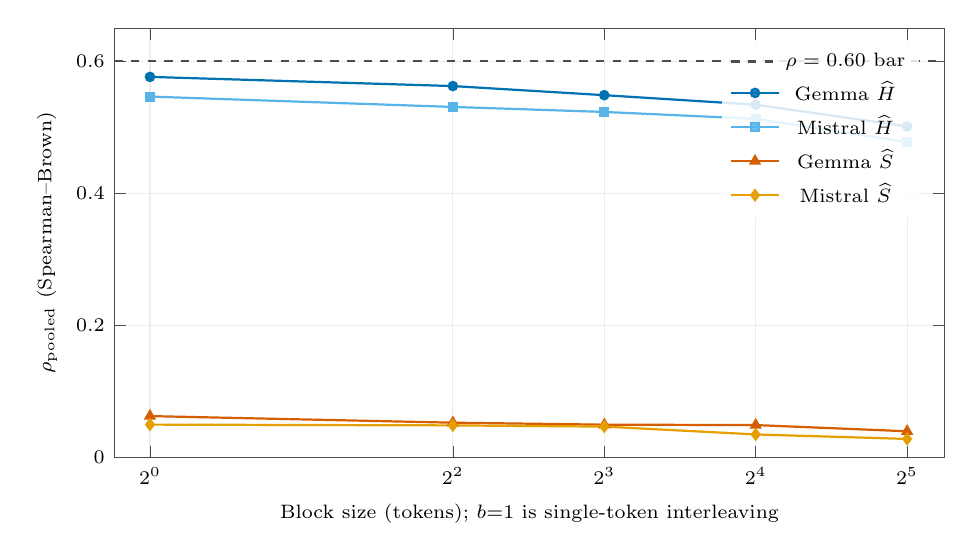
\begin{tikzpicture}
\begin{axis}[
  width=\linewidth, height=0.58\linewidth,
  xmode=log, log basis x=2,
  xlabel={Block size (tokens); $b{=}1$ is single-token interleaving},
  ylabel={$\rho_{\mathrm{pooled}}$ (Spearman--Brown)},
  xmin=0.85, xmax=38, ymin=0, ymax=0.65,
  xtick={1,4,8,16,32},
  ytick={0,0.2,0.4,0.6},
  grid=major, grid style={gray!15},
  legend style={font=\scriptsize, at={(0.97,0.97)}, anchor=north east, draw=none,
                fill=white, fill opacity=0.85, text opacity=1},
  tick label style={font=\scriptsize}, label style={font=\scriptsize},
  axis line style={draw=inkGrey}, tick style={draw=inkGrey},
]
\addplot[domain=0.85:38, samples=2, dashed, thick, color=inkGrey] {0.60};
\addlegendentry{$\rho=0.60$ bar}
\addplot[color=okBlue, mark=*, mark size=1.5pt, thick] coordinates {
 (1,0.5763)(4,0.5624)(8,0.5486)(16,0.5342)(32,0.5013)
};
\addlegendentry{Gemma $\Hest$}
\addplot[color=okSky, mark=square*, mark size=1.4pt, thick] coordinates {
 (1,0.5465)(4,0.5308)(8,0.5232)(16,0.5128)(32,0.4777)
};
\addlegendentry{Mistral $\Hest$}
\addplot[color=okVermil, mark=triangle*, mark size=1.8pt, thick] coordinates {
 (1,0.0626)(4,0.0526)(8,0.0496)(16,0.0490)(32,0.0396)
};
\addlegendentry{Gemma $\Sest$}
\addplot[color=okOrange, mark=diamond*, mark size=1.8pt, thick] coordinates {
 (1,0.0497)(4,0.0485)(8,0.0467)(16,0.0348)(32,0.0280)
};
\addlegendentry{Mistral $\Sest$}
\end{axis}
\end{tikzpicture}

\caption{Reliability against block size, $b=1$ is single-token interleaving.
The decline is smooth and monotonic in the direction that argues
\emph{against} the sequence-geometry objection: coarser blocks, which decimate
the sequence less, are systematically \emph{less} reliable, not more.
Source: \texttt{review\_results/data/t0\_t1\_MERGED\_table.json}.}
\label{fig:splitconstruction}
\end{figure}

\begin{table}[h]
\centering
\footnotesize
\caption{Split-half reliability ($\rho_{\text{pooled}}$) under all eight tested
constructions. \texttt{block\_$b$} assigns contiguous blocks of $b$ tokens
alternately to the two halves, so \texttt{interleave} is the $b\!=\!1$ case and
\texttt{contiguous} the single-block limit. \texttt{block\_bootstrap} is measured but structurally invalid
here: its two halves share $\approx\!47\%$ of token positions by construction
(block length $\ge\!96$ on a $\approx\!400$-token document), so its inflated
correlation reflects token overlap, not document-level signal, and it is
excluded from the headline claim. \texttt{permutation} is the median of $20$
random-membership replicates (order preserved within each half), $[$p5,p95$]$
in brackets. Source: \texttt{review\_results/data/t0\_t1\_MERGED\_table.json},
\texttt{t1\_permutation\_stats.json}.}
\label{tab:splitconstruction}
\resizebox{\linewidth}{!}{%
\begin{tabular}{lrrrr}
\toprule
Construction & \texttt{gemma\_H} & \texttt{gemma\_S} & \texttt{mistral\_H} & \texttt{mistral\_S} \\
\midrule
interleave (headline)         & 0.5763 & 0.0626 & 0.5465 & 0.0497 \\
block\_4                      & 0.5624 & 0.0526 & 0.5308 & 0.0485 \\
block\_8                      & 0.5486 & 0.0496 & 0.5232 & 0.0467 \\
block\_16                     & 0.5342 & 0.0490 & 0.5128 & 0.0348 \\
block\_32                     & 0.5013 & 0.0396 & 0.4777 & 0.0280 \\
contiguous (pre-registered as confounded) & 0.2609 & 0.0159 & 0.2678 & 0.0040 \\
permutation, $20$ reps (median \ci{p5}{p95}) & 0.5443\,\ci{.5424}{.5462} & 0.0530\,\ci{.0484}{.0571} & 0.5152\,\ci{.5129}{.5182} & 0.0452\,\ci{.0386}{.0498} \\
matched\_sweep (full $6$-value \texttt{WINDOW\_SCALE}) & 0.5763 & 0.0626 & 0.5465 & 0.0497 \\
\midrule
\texttt{block\_bootstrap} (excluded, see caption) & 0.7779\rlap{$^\dagger$} & 0.2047\rlap{$^\dagger$} & 0.7769\rlap{$^\dagger$} & 0.1912\rlap{$^\dagger$} \\
\bottomrule
\end{tabular}}
\end{table}

\paragraph{The headline robustness test.} The plan's own pre-registered bar
asks whether \texttt{gemma\_S} stays inside $[0.03,0.12]$ across every valid
construction. It does not: \texttt{contiguous} falls to $0.0159$. That is the
\emph{expected} signature of the drift confound the interleaved design was
built to avoid --- \texttt{gemma\_H} collapses in the same construction,
$0.576\to0.261$, consistent with genuine within-document stylistic drift
entering a contiguous split and not the other constructions --- so it is read
as confirming, not undermining, the case for interleaving. The five
remaining valid constructions (interleave, four block sizes, the permutation
median and the matched full sweep) span $0.0396$--$0.0626$, comfortably inside
the band.

\paragraph{An order-scrambling construction, kept as a diagnostic.} Among the
constructions swept for the permutation check is one built from an
\emph{unsorted} random index set for each half, which scrambles a half's
internal token order along with its membership. Because both estimators are
functionals of ordered structure, this construction collapses $\rho$ to
$\approx\!0.003$ for every quantity, in sharp contrast to every order-preserving
construction tested. We keep it here as a direct demonstration that these
quantities are genuinely order-dependent --- destroying order destroys the
signal, which a magnitude or length statistic computed on the same tokens
would not do.

\subsection{Variance decomposition (Route 1 and Route 2)}
\label{app:variancecomponents}

Route 1 demeans both halves by their own $(\text{class},\text{domain},\text{temp})$
stratum before correlating --- the number quoted in \S\ref{sec:background} as
$\rho_{\text{within}}$. Route 2 is a closed-form, one-way variance-components
decomposition (method-of-moments, not an iterative mixed model, chosen for zero
convergence risk at $n\!\approx\!223{,}834$) that additionally reports the
population share and a cluster-robust standard error, clustered by seed
article.

\begin{table}[h]
\centering
\footnotesize
\caption{Variance decomposition. ICC is the fraction of single-half variance
explained by $(\text{class},\text{domain},\text{temp})$ stratum membership,
i.e.\ an estimate of $\mathrm{Var}(\mu)/(\mathrm{Var}(\mu)+\mathrm{Var}(\delta)+\mathrm{Var}(\eta))$.
Source: \texttt{review\_results/data/t0\_variance\_components.json}.}
\label{tab:variancecomponents}
\begin{tabular}{lrrrrr}
\toprule
Quantity & $\rho_{\text{pooled}}$ & $\rho_{\text{within}}$ & ICC & $\mathrm{Var}(\delta)$ & cluster-robust SE \\
\midrule
\texttt{gemma\_H}   & 0.576 & 0.552 & 3.9\%  & 0.00217 & 0.0023 \\
\texttt{mistral\_H} & 0.547 & 0.520 & 3.9\%  & 0.00190 & 0.0024 \\
\texttt{gemma\_S}   & 0.063 & 0.060 & 0.14\% & 0.01049 & 0.0024 \\
\texttt{mistral\_S} & 0.050 & 0.046 & 0.18\% & 0.00870 & 0.0023 \\
\bottomrule
\end{tabular}
\end{table}

Reading the two exponents side by side: for \Hest, population structure
(class, domain, temperature together) explains only $\approx\!4\%$ of
single-half variance, so the $0.576\to0.552$ drop is real but modest --- most
of what \S\ref{sec:reliability} measures for \Hest\ was already
within-population. For \Sest, population structure explains under $0.2\%$ of
variance: \Sest's poor pooled reliability is essentially all within-document
estimation noise, ruling out ``pooling across populations inflates apparent
unreliability'' as an explanation for \Sest\ either way. \emph{Note}: GAGLE has
no generator column distinct from \texttt{Label} (Human/Gemma-2B/Mistral-7B
already is the class--generator join), so the demeaning set is
$(\text{Label},\text{domain},\text{temp})$ throughout --- the same information
content as $(\text{class},\text{generator},\text{domain},\text{temp})$, without
a redundant fourth column. Prompt type is deliberately excluded from the
demeaning set throughout this appendix, because \S\ref{sec:withinpop} treats
what is predictable from prompt type as part of $\delta$; demeaning by it here
would remove the very quantity that section measures.

\subsection{Reliability as a function of support, and $N^{\star}$}
\label{app:nstar}

The construction behind \S\ref{sec:reliability}'s $N^{\star}$ claim. An
estimator noise floor $\mathrm{Var}(\eta_N)$ is calibrated against synthetic
fractional Gaussian noise (Davies--Harte generator) at $\Htrue\in\{0.60,0.65,0.70,0.72\}$,
averaged to match GAGLE's own observed $\Hest$ band; $\mathrm{Var}(\delta)$ is
taken from Table~\ref{tab:variancecomponents}; and
$\rho_{\text{SB}}(N)=2r(N)/(1+r(N))$ for
$r(N)=\mathrm{Var}(\delta)/(\mathrm{Var}(\delta)+\mathrm{Var}(\eta_N))$ is
composed at each grid point $N\in\{100,200,400,800,1600,3200,6400,12800\}$.
$N^{\star}$ is the first grid point at which $\rho_{\text{SB}}(N)$ crosses
$0.60$; the true crossing may lie between grid points.

\begin{figure}[h]
\centering
% =============================================================================
%  fig_nstar.tex -- reliability as a function of support, and where it crosses
%  the pre-registered 0.60 bar. Every coordinate below is read directly from
%  review_results/data/t2_n_star_composition.json (fBm noise-floor calibration
%  at GAGLE's own observed H in [0.60,0.72], Var(delta) from the T0 decomposition,
%  rho_SB = 2r/(1+r) composed at each N). None is illustrative or interpolated
%  beyond the plotted grid points, which are joined by straight segments only.
% =============================================================================
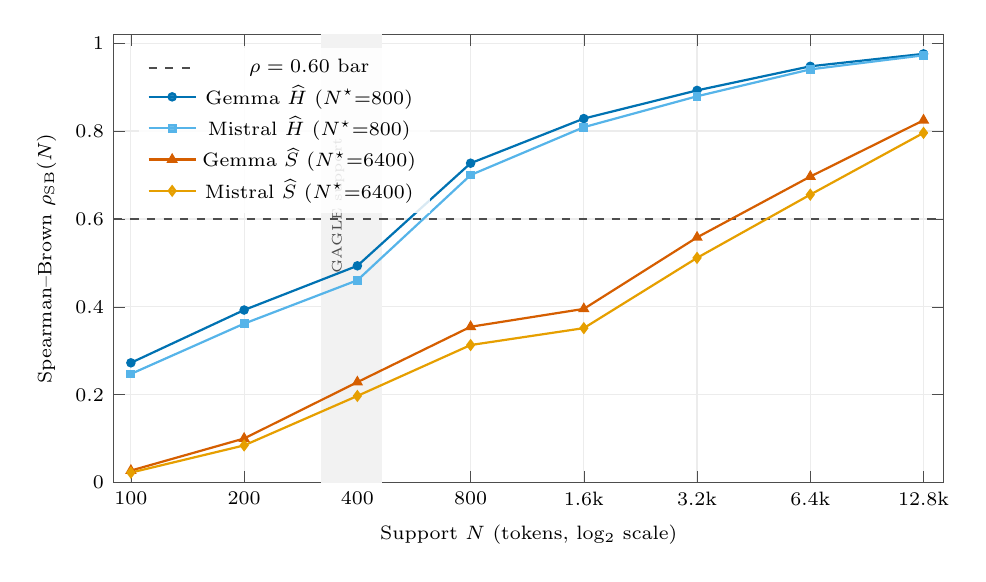
\begin{tikzpicture}
\begin{axis}[
  width=\linewidth, height=0.60\linewidth,
  xmode=log, log basis x=2,
  xlabel={Support $N$ (tokens, log$_2$ scale)},
  ylabel={Spearman--Brown $\rho_{\mathrm{SB}}(N)$},
  xmin=90, xmax=14500, ymin=0, ymax=1.02,
  xtick={100,200,400,800,1600,3200,6400,12800},
  xticklabels={100,200,400,800,{1.6k},{3.2k},{6.4k},{12.8k}},
  ytick={0,0.2,0.4,0.6,0.8,1.0},
  grid=major, grid style={gray!15},
  legend style={font=\scriptsize, at={(0.03,0.97)}, anchor=north west, draw=none,
                fill=white, fill opacity=0.85, text opacity=1, row sep=-1pt},
  tick label style={font=\scriptsize}, label style={font=\scriptsize},
  axis line style={draw=inkGrey}, tick style={draw=inkGrey},
  clip=false,
]
% GAGLE's own usable-token band (320-464), shaded, drawn first so it sits behind data
\draw[fill=softGrey, draw=none] (axis cs:320,0) rectangle (axis cs:464,1.02);
\node[font=\tiny, text=inkGrey, rotate=90, anchor=south] at (axis cs:392,0.63) {GAGLE support};
% pre-registered bar
\addplot[domain=90:14500, samples=2, dashed, thick, color=inkGrey] {0.60};
\addlegendentry{$\rho=0.60$ bar}
% series
\addplot[color=okBlue, mark=*, mark size=1.3pt, thick] coordinates {
 (100,0.2727)(200,0.3928)(400,0.4934)(800,0.7268)(1600,0.8284)(3200,0.8925)(6400,0.9473)(12800,0.9756)
};
\addlegendentry{Gemma $\Hest$ ($N^{\star}{=}800$)}
\addplot[color=okSky, mark=square*, mark size=1.2pt, thick] coordinates {
 (100,0.2474)(200,0.3618)(400,0.4605)(800,0.6999)(1600,0.8088)(3200,0.8791)(6400,0.9403)(12800,0.9723)
};
\addlegendentry{Mistral $\Hest$ ($N^{\star}{=}800$)}
\addplot[color=okVermil, mark=triangle*, mark size=1.6pt, thick] coordinates {
 (100,0.0275)(200,0.1005)(400,0.2287)(800,0.3547)(1600,0.3954)(3200,0.5580)(6400,0.6964)(12800,0.8245)
};
\addlegendentry{Gemma $\Sest$ ($N^{\star}{=}6400$)}
\addplot[color=okOrange, mark=diamond*, mark size=1.6pt, thick] coordinates {
 (100,0.0229)(200,0.0848)(400,0.1973)(800,0.3131)(1600,0.3516)(3200,0.5114)(6400,0.6553)(12800,0.7958)
};
\addlegendentry{Mistral $\Sest$ ($N^{\star}{=}6400$)}
\end{axis}
\end{tikzpicture}

\caption{Reliability against support, calibrated fBm noise floor.
Shaded band: GAGLE's own $320$--$464$-token usable-support range. \Hest\ (blue,
sky) crosses $\rho=0.60$ near $N{=}800$; \Sest\ (vermillion, orange) does not
cross until $N{=}6{,}400$. Source: \texttt{review\_results/data/t2\_n\_star\_composition.json}.}
\label{fig:nstar}
\end{figure}

\begin{table}[h]
\centering
\footnotesize
\caption{$N^{\star}$: first grid point where the calibrated $\rho_{\text{SB}}(N)$
crosses $0.60$. Full curve (all eight grid points) in
\texttt{review\_results/data/t2\_n\_star\_composition.json}.}
\label{tab:nstar}
\begin{tabular}{lrrr}
\toprule
Quantity & $\mathrm{Var}(\delta)$ & $\rho_{\text{SB}}$ at $N{=}400$ & $N^{\star}$ \\
\midrule
\texttt{gemma\_H}   & 0.00217 & 0.493 & \textbf{800} \\
\texttt{mistral\_H} & 0.00190 & 0.460 & \textbf{800} \\
\texttt{gemma\_S}   & 0.01049 & 0.229 & \textbf{6{,}400} \\
\texttt{mistral\_S} & 0.00870 & 0.197 & \textbf{6{,}400} \\
\bottomrule
\end{tabular}
\end{table}

\paragraph{What the real-text bracket does and does not establish.} A
companion pass measures within-document block variance of \Hest/\Sest\ across
disjoint $N$-token blocks on $5{,}000$ full-length human documents (uncapped up
to the corpus's own $2{,}047$-token limit). At the matched $N$ values this
real-text variance runs at or below the calibrated fBm floor (e.g.\ at $N=400$:
\Sest\ variance $0.0603$ real-text against $0.0707$ fBm; \Hest\ variance
$0.0046$ against $0.0045$, materially the same). An earlier draft of this
analysis read that gap as an upper bound on $\mathrm{Var}(\eta_N)$; it is not
--- blocks drawn from one document share that document's own realisation,
which suppresses between-block variance relative to the independent draws the
fBm floor uses, an effect distinct from and opposed to the nonstationarity a
bound argument would need. What the bracket \emph{does} establish, via a
calibration check (median full-document $\Hest=0.629$ across all $5{,}000$
documents, squarely inside the $0.60$--$0.72$ calibration band), is that the
fBm floor is not an underestimate of real-text estimator scatter \emph{for
\Hest}. \textbf{The check does not extend to \Sest, and there the floor is
measurably optimistic}: the composed $\rho_{\text{SB}}(400)$ of
$0.229$/$0.197$ (Table~\ref{tab:nstar}) sits $3.7$--$4.0\times$ above the
$0.063$/$0.050$ measured at the same support (Table~\ref{tab:appreliability}),
so it understates $\mathrm{Var}(\eta_{400})$ for \Sest. $N^{\star}$ is
therefore a point estimate under a validated floor for \Hest, and a
\emph{lower} bound for \Sest: correcting the floor moves \Sest's crossing
further out, never nearer.
% source: review_results/data/t2_step1_noise_floor.json; t2_step2_real_text_bracket.json; t2_step2_full_doc_estimates.json

\subsection{Estimator invariance, part 1: detrended fluctuation analysis and local Whittle}
\label{app:altestimators}

This appendix and the persistent-homology pilot of Appendix~\ref{app:limitations}
(``Estimator invariance, part 2'') ask the same question with three
structurally different tools: is the short-support reliability ceiling a
property of \emph{what} is being measured, or an artifact of \emph{how} one
particular estimator measures it? DFA and the local-Whittle spectral estimator
are each designed, for different reasons, to be more robust than the plain
rescaled-range (R/S) statistic used as this paper's headline to the kind of
non-stationarity a short, topically drifting document introduces. DFA fits and
subtracts a local polynomial trend from the surprisal walk before measuring
its fluctuation at each scale, so slow within-document drift does not get
folded into the exponent; the local-Whittle estimator instead works in the
frequency domain, fitting the low-frequency slope of the sequence's power
spectrum, which is less sensitive to a handful of extreme surprisal spikes
than a windowed range statistic is. If either recovers substantially higher
reliability than R/S at the same support, the ceiling would be an R/S
artifact rather than a property of the estimand; if not, it generalises.

Refitting DFA (order-$1$, same scale sweep) and a local-Whittle spectral
estimator on the identical interleaved halves used throughout this appendix.

\begin{table}[h]
\centering
\footnotesize
\caption{Reliability by estimator. \texttt{passes} marks $\rho\ge0.60$.
Local-Whittle saturation (its bounded optimiser hitting $[-0.49,1.49]$) affects
$0.0001$ of pairs for both scorers and moves reliability by $<0.001$ when
excluded --- not the source of its clearance.
Source: \texttt{review\_results/data/t4\_alt\_estimators\_reliability.json}.}
\label{tab:altestimators}
\begin{tabular}{lrrrl}
\toprule
Quantity & $n$ & $\rho_{\text{pooled}}$ & $\rho_{\text{within}}$ & Passes $0.60$? \\
\midrule
\texttt{gemma\_RS\_H} (headline)   & 221{,}904 & 0.576 & 0.552 & no \\
\texttt{gemma\_DFA\_H}             & 221{,}904 & 0.629 & 0.601 & \textbf{yes (by 0.029)} \\
\texttt{gemma\_Whittle\_H}         & 221{,}904 & 0.677 & 0.647 & \textbf{yes} \\
\texttt{mistral\_RS\_H} (headline) & 223{,}834 & 0.547 & 0.520 & no \\
\texttt{mistral\_DFA\_H}           & 223{,}834 & 0.599 & 0.566 & no (by 0.0006) \\
\texttt{mistral\_Whittle\_H}       & 223{,}834 & 0.642 & 0.605 & \textbf{yes} \\
\bottomrule
\end{tabular}
\end{table}

\begin{table}[h]
\centering
\footnotesize
\caption{Cross-estimator correlation, document level (mean of halves).
Thresholds fixed before this table was produced: $>0.85$ reads as ``the same
quantity, more precisely measured''; $<0.60$ reads as ``a different quantity''.
Source: same file as Table~\ref{tab:altestimators}.}
\label{tab:crossestimator}
\begin{tabular}{lrr}
\toprule
Pair & Gemma & Mistral \\
\midrule
R/S $\sim$ DFA     & 0.869 & 0.864 \\
R/S $\sim$ Whittle  & 0.759 & 0.751 \\
DFA $\sim$ Whittle & 0.808 & 0.803 \\
\bottomrule
\end{tabular}
\end{table}

R/S and DFA clear the ``same quantity'' threshold ($0.86$--$0.87$): DFA is a
less-noisy estimator of the same Hurst exponent, and its clearance of $0.60$ is
real but marginal and scorer-dependent, which is why \S\ref{sec:reliability}
reports it as ``at the margin'' rather than as unqualified recoverability. R/S
and Whittle correlate more weakly ($0.75$--$0.76$), so Whittle's more
comfortable clearance ($0.677$/$0.642$) is partly a different quantity, not
purely a cleaner measurement of the same one, and is reported here alongside
this correlation rather than as a standalone headline. Neither estimator has a
literature-standard analogue for \Sest's displacement-probability construction;
\Sest's reliability is unaffected by this appendix and stands exactly where
\S\ref{sec:reliability} puts it.

Part 2 of this argument, on a representation with no scale-exponent machinery
at all, is in Appendix~\ref{app:limitations} (``Estimator invariance, part
2''): a persistent-homology pilot on token-embedding trajectories hits the
same short-support wall by an entirely different route --- evidence for the
mechanism itself, not for an artifact of any one estimator's implementation.

% -----------------------------------------------------------------------------
\section{Extended Detection Results}
\label{app:detection}

\paragraph{Harness controls.} The label-shuffle control runs the full harness on
permuted training labels and lands systematically \emph{below} chance --- mean AUROC
$0.3693$ (sd $0.0427$) on the random fold, $0/10$ permutations above $0.5$, and all
eight folds pass a one-sided criterion --- because human rows occupy a sparse extreme
region of the feature space that a class-weighted booster on random labels assigns
the global prior. Injecting leakage raises it monotonically and past the decision
boundary at every non-zero level tested ($0\%\!:0.4166$; $2\%\!:0.5080$;
$5\%\!:0.5534$; $20\%\!:0.8019$), so the control detects what it exists to detect,
and its sensitivity floor sits below a $2\%$ contamination rather than above $5\%$.
This catches a class of failure --- an index misalignment, or a metric computed
against the wrong vector --- that no confound configuration could, because all five
would be wrong together.
% source: findings/results/p3_tables.md, "Harness control -- label shuffle"

\paragraph{Multiplicity, and the learner check.} Across all forty paired tests (five
configurations $\times$ eight folds) DeLong and the paired bootstrap agree in $40$ of
$40$, and Holm--Bonferroni leaves \emph{three} survivors, all on the
\texttt{billsum} fold and cutting both ways --- two where fractal features are
significantly worse ($p=9.4\!\times\!10^{-9}$, $p=3.2\!\times\!10^{-5}$) and one
where they are significantly better ($p=4.6\!\times\!10^{-5}$), across three
configurations. A cross-fold ``fractal is significantly harmful'' framing does not
survive correction; what survives is narrower and more interesting --- the effect is
statistically real only where the domain shift is largest, and its sign there depends
on how missingness is handled. The sole cell favouring the full model,
\texttt{lodo/big\_patent}, does so by $0.0001$ AUROC, inside that cell's own
bootstrap width. The result is not an artifact of the learner: a shallow multilayer
perceptron (one hidden layer, $64$ units, imputed and scaled, class-balanced) trails
the tree ensemble on all eight folds and collapses to TPR@$1\%$FPR $=0.0000$ on two
of them, where the tree ensemble never does, and the fractal family does not rescue
it.
% source: reports/2026-08-25_writeup_flags_and_limitations.md entry 10;
%         findings/results/p0_p5_audit.md S3.2

\paragraph{The substitution test, per fold.} Isolating a nine-feature log-perplexity
group and running \arm{fractal+logppl} ($63$ features) against \arm{stat\_only}
($17$) on population-matched folds, the fractal arm loses on all eight of eight
folds on both AUROC and TPR@$1\%$FPR: $0.9684/0.6460$ against $0.9795/0.7289$
in-distribution, and $0.8191/0.2050$ against $0.8735/0.3171$ on \texttt{billsum}
LODO. Swapping fractal features \emph{in} for entropy and rank statistics, at
comparable combination shape, makes every fold worse.
% source: findings/results/p0_p5_audit.md S3.3

\begin{table}[h]
\centering
\caption{Feature-family ablation, in-distribution (random split, \arm{full}),
$n_{\text{test}}=43{,}413$, human prevalence $2.23\%$, $2{,}000$-fold stratified
bootstrap. Remaining arms and all eight folds: Appendix~\ref{app:detection}.}
\label{tab:ablation}
\footnotesize
\resizebox{\linewidth}{!}{%
\begin{tabular}{lrccl}
\toprule
Arm & \#feat & AUROC & TPR@$1\%$FPR & Reading \\
\midrule
\arm{fractal\_only}      & 54 & \textcolor{okVermil}{0.6629} \ci{.6458}{.6782} & 0.0641 \ci{.0429}{.0914} & real signal, far below either baseline \\
\arm{stat\_only}         & 17 & 0.9795 & 0.7209 & incumbent: perplexity, entropy, ranks \\
\arm{style\_only}        & 14 & 0.9919 & 0.7964 & incumbent: discourse and surface form \\
\arm{fractal+stat}       & 71 & 0.9785 & 0.6836 & \emph{below} \arm{stat\_only} on both \\
\arm{all}                & 85 & 0.9984 \ci{.9976}{.9990} & 0.9587 \ci{.9489}{.9738} & full model \\
\arm{all\_minus\_fractal}& 31 & \textcolor{okGreen}{0.9984} & \textcolor{okGreen}{0.9612} \ci{.9360}{.9781} & \textbf{all 54 fractal features deleted} \\
\bottomrule
\end{tabular}}
\end{table}

\paragraph{Remaining arms.} Three arms omitted from Table~\ref{tab:ablation} for
space: \arm{fractal+style} ($68$ features) reaches AUROC $0.9917$ / TPR@$1\%$FPR
$0.8171$, within noise of \arm{style\_only} on AUROC; \arm{all\_minus\_length}
($83$) reaches $0.9974$/$0.9436$, so removing length costs $0.0010$ AUROC and
$0.0151$ TPR@$1\%$FPR; and \arm{length\_only} ($2$) reaches $0.8635$/$0.0477$, a
partial detector of \emph{human} text and the priced form of the corpus's dominant
confound. Four further diagnostic arms,
each of which declared a failure condition in advance, on the same random split
and \arm{full} configuration: \arm{provenance\_only} reaches
AUROC $0.5655$ / TPR@$1\%$FPR $0.1196$ on the six window-length provenance
columns, which prices that exclusion (the eleven exit-gate flags are a
separate, disjoint set); \arm{shortwindow\_only} ($2$) reaches
$0.5290$/$0.0580$, weakly predictive and demonstrably unused;
\arm{missingness\_only} ($85$) reaches $0.5169$/$0.0305$, the missingness
pattern alone; and \arm{label\_shuffle} lands at $0.3693$ with $0/10$
permutations above chance.
% source: findings/results/p3_tables.md, RANDOM config 1

\begin{table}[h]
\centering
\footnotesize
\caption{\arm{all} versus \arm{all\_minus\_fractal} on all eight frozen
group-disjoint folds, \arm{full} configuration: one random in-distribution
split, five leave-one-domain-out (LODO) and two leave-one-generator-out (LOGO).
Each fold is scored on the frozen test split of its held-out stratum, which is
why the LOGO $n$ is a fraction of that generator's corpus count rather than all
of it. AUROC at six decimals to make
the ties legible. \arm{all\_minus\_fractal} ties or wins on $7$ of $8$.
Source: \texttt{data/p3\_t1\_results.json};
\texttt{reports/2026-08-30\_fractalscope\_verification\_checks.md} \S2.}
\label{tab:folds}
\begin{tabular}{llrrrrl}
\toprule
Scheme & Held-out fold & $n_{\text{test}}$ & \arm{all} (85) & \arm{a-m-f} (31)
       & $\Delta$ & Winner \\
\midrule
random & ---                        & 43{,}413 & 0.998397 & 0.998397 & $+1.5\!\times\!10^{-7}$ & tie \\
lodo   & \texttt{big\_patent}       & 45{,}175 & 0.998571 & 0.998468 & $-0.000103$ & \arm{all} \\
lodo   & \texttt{billsum}           & 45{,}146 & 0.937608 & 0.941725 & $+0.004117$ & no-fractal \\
lodo   & \texttt{newsroom}          & 44{,}718 & 0.992131 & 0.992077 & $-0.000054$ & tie \\
lodo   & \texttt{scientific\_papers}& 43{,}749 & 0.994487 & 0.995077 & $+0.000590$ & no-fractal \\
lodo   & \texttt{wikipedia}         & 45{,}046 & 0.987009 & 0.987990 & $+0.000981$ & no-fractal \\
logo   & \texttt{gemma\_2b}         & 22{,}747 & 0.987404 & 0.988510 & $+0.001106$ & no-fractal \\
logo   & \texttt{mistral\_7b}       & 21{,}635 & 0.986638 & 0.987624 & $+0.000986$ & no-fractal \\
\bottomrule
\end{tabular}
\end{table}

\begin{table}[h]
\centering
\footnotesize
\caption{AUROC / TPR@$1\%$FPR, \arm{full} configuration, gradient-boosted tree,
all arms on the seven shifted folds.
Source: \texttt{results/p3\_tables.md}, LODO and LOGO config 1.}
\label{tab:appfolds}
\resizebox{\linewidth}{!}{%
\begin{tabular}{llcccccc}
\toprule
& & \arm{fractal} & \arm{stat} & \arm{style} & \arm{all} & \arm{a-m-f} & \arm{length} \\
Scheme & Fold & (54) & (17) & (14) & (85) & (31) & (2) \\
\midrule
lodo & \texttt{big\_patent}        & .6274/.0278 & .9626/.6034 & .9907/.7617 & .9986/.9632 & .9985/.9539 & .9734/.2636 \\
lodo & \texttt{billsum}            & .5278/.0311 & .8732/.3235 & .8797/.0612 & .9376/.4931 & .9417/.5031 & .7234/.0177 \\
lodo & \texttt{newsroom}           & .6624/.0406 & .9858/.8143 & .9385/.3570 & .9921/.8921 & .9921/.8847 & .7566/.0077 \\
lodo & \texttt{scientific\_papers} & .6968/.0913 & .9810/.7705 & .9851/.6336 & .9945/.8769 & .9951/.8918 & .9529/.0819 \\
lodo & \texttt{wikipedia}          & .5984/.0464 & .9667/.7245 & .9561/.4518 & .9870/.8178 & .9880/.8345 & .8132/.0359 \\
logo & \texttt{gemma\_2b}          & .6163/.0531 & .9004/.4171 & .9786/.6112 & .9874/.7954 & .9885/.8079 & .8506/.0333 \\
logo & \texttt{mistral\_7b}        & .6567/.0746 & .9089/.4114 & .9810/.7065 & .9866/.7419 & .9876/.7555 & .8549/.0555 \\
\bottomrule
\end{tabular}}
\end{table}

Two patterns in Table~\ref{tab:appfolds} are worth naming. First,
\arm{fractal\_only} is at or near chance on the hardest fold (\texttt{billsum},
AUROC $0.5278$) and never exceeds $0.6968$ anywhere. Second, the incumbent
families trade places by domain --- \arm{style\_only} leads on
\texttt{big\_patent} and \texttt{scientific\_papers}, \arm{stat\_only} on
\texttt{newsroom} --- the signature of a detector whose components are
domain-sensitive in different directions, and part of why the fused model holds
up better than any single family.

\paragraph{The \texttt{billsum} LODO error analysis.} The hardest fold shows the
failure mode the whole $85$-feature representation has, independent of the
fractal family. AUROC falls only to $0.9376$ while TPR@$1\%$FPR falls to
$0.4931$ --- a tail-ranking failure, not a calibration artifact: bulk ranking is
preserved and the extreme tail is not. An error analysis on this fold (run on a
refit whose headline cell was $0.9476$/$0.5630$, before a later
feature-tokenisation correction moved it to the values quoted above; the
mechanism, not the level, is what carries forward)
% source: reports/2026-08-25_P3_error_analysis_billsum_LODO_collapse.md
finds the driver is prompt type by a wide margin. False-negative rate runs
$0.677$ for chain-of-thought, $0.676$ for excerpt continuation and $0.608$ for
pretrained continuation, against $0.259$--$0.350$ for keyword- and
summary-constrained generation --- a $1.7$--$2.6\times$ gap. Freely generated
text on this domain's legal-summary register reads closer to human. The largest
distributional shifts into this fold are style features
(\texttt{Sent\_Len\_Std} $+0.595$ standardised, KS $0.255$;
\texttt{Bigram\_Repetition\_Rate} $+0.263$) --- the family carrying $63.46\%$ of
the model's gain.

\paragraph{Deployment-operating-point diagnostics.} Beyond the ranking metrics
above, three questions bear on deployment: how the detector behaves at very
low false-positive budgets, whether its threshold calibration holds under
resampling, and how precision changes with the assumed prevalence of
LLM-generated text in the traffic being screened. On the \arm{full}
configuration random split ($n=43{,}413$), partial AUROC restricted to
FPR$\le1\%$ is $0.9595$ and to FPR$\le5\%$ is $0.9857$; TPR at a fixed $5\%$
FPR threshold is $0.9952$, and at a much stricter $0.1\%$ FPR threshold falls
to $0.6729$ (point estimate, $2{,}000$-fold bootstrap). Re-deriving the
operating threshold on resampled folds and checking the FPR it actually
achieves against its $1\%$ and $5\%$ targets gives $0.93\%$ $[0.41\%,1.55\%]$
and $4.95\%$ $[3.61\%,6.40\%]$ respectively --- both targets covered within
CI, so the thresholds in Table~\ref{tab:ablation} are not overfit to one
split. Expected calibration error (15 equal-width bins) is $0.00091$: the
model's predicted probabilities track observed frequencies closely at this
operating point.
% source: review_results/data/t8_deployment_metrics.json

GAGLE's own corpus is $97.77\%$ LLM-generated (human text is the rare class
by construction of the benchmark); a real moderation deployment is typically
the opposite shape, with LLM-generated content the minority of traffic.
Because precision is prevalence-dependent even when AUROC is not,
Table~\ref{tab:ppv} reports PPV at the $1\%$- and $5\%$-FPR thresholds across
a range of \emph{assumed} LLM prevalence in deployment traffic, not GAGLE's
own training prevalence, up to GAGLE's own composition as a reference point.

\begin{table}[h]
\centering
\footnotesize
\caption{Positive predictive value at fixed FPR thresholds, by assumed
LLM-content prevalence in deployment traffic (distinct from GAGLE's own
training-corpus composition, bottom row, included as a reference point).
Each cell is
$\mathrm{PPV}=\mathrm{TPR}\,\pi/\big(\mathrm{TPR}\,\pi+\mathrm{FPR}(1-\pi)\big)$
at the achieved FPRs ($0.93\%$ and $4.95\%$), with $\pi$ the assumed prevalence.
\arm{full} configuration, random split.}
\label{tab:ppv}
\begin{tabular}{lcc}
\toprule
Assumed LLM share of traffic & PPV @ $1\%$FPR & PPV @ $5\%$FPR \\
\midrule
$1\%$  & 0.510 & 0.169 \\
$5\%$  & 0.845 & 0.514 \\
$10\%$ & 0.920 & 0.691 \\
$25\%$ & 0.972 & 0.870 \\
$50\%$ & 0.990 & 0.953 \\
$97.77\%$ (GAGLE's own composition) & 0.9998 & 0.999 \\
\bottomrule
\end{tabular}
\end{table}
% source: review_results/data/t8_deployment_metrics.json

% -----------------------------------------------------------------------------
\section{Feature Importance Accounting}
\label{app:importance}

Split gain and permutation importance are reported together throughout, because
they disagree. Table~\ref{tab:gain} gives the family totals; the per-column
table for all $85$ inputs, including every zero-contribution column, is in
\texttt{results/p3\_tables.md}. Reporting only the columns that worked is the
selective reporting the pre-declared reporting rule exists to prevent, so every
declared feature appears there, and none has exactly zero gain.

\begin{table}[h]
\centering
\footnotesize
\caption{Gain versus permutation accounting, \arm{all} arm, random split.
Permutation importance is the AUROC drop when a column is shuffled on the test
fold, five repeats. Source: \texttt{results/p3\_tables.md} (D-13).}
\label{tab:gain}
\begin{tabular}{lrrrrr}
\toprule
Family & \#feat & total split gain & gain share & summed perm.\ drop & perm.\ share \\
\midrule
style    & 14 & 1{,}296{,}092.4 & 63.46\% & $2.04\times10^{-2}$ & 56.7\% \\
stat     & 17 &    633{,}456.7  & 31.02\% & $1.54\times10^{-2}$ & 42.8\% \\
fractal  & 54 &    112{,}761.3  &  5.52\% & $\mathbf{1.7\times10^{-4}}$ & \textbf{0.47\%} \\
\bottomrule
\end{tabular}
\end{table}

\paragraph{Per-column detail.} Only two fractal columns appear in the top $25$ by
gain. The highest, \texttt{Gemma\_H}, ranks $23$rd with $0.28\%$ of gain and a
permutation drop of $3\!\times\!10^{-5}\pm3\!\times\!10^{-5}$; for comparison the
top column overall, \texttt{N\_Words\_Used}, has $39.99\%$ of gain and a drop of
$1.28\!\times\!10^{-2}\pm2.1\!\times\!10^{-4}$. The two cross-scorer divergence
features --- the design's explicit attempt to extract signal from
\emph{disagreement} between a $2$B and a $7$B scorer's estimates on the same
document --- rank $60$th and $68$th of $85$.

\paragraph{Distribution within the fractal family.} All $54$ columns have a
permutation drop below $10^{-4}$. Thirty-five are zero or negative --- shuffling
them improves held-out AUROC --- and thirty-eight lie within their own standard
error of zero. The highest-ranked fractal column by gain is \texttt{Gemma\_H} at
overall rank $23$ ($0.28\%$ gain, $237$ splits, permutation drop
$3\times10^{-5}\pm3\times10^{-5}$); the lowest is
\texttt{Mistral\_S\_window\_max} at rank $85$. Only two fractal columns appear
in the top $25$.

\paragraph{Reading the disagreement.} Gain counts splits weighted by local
objective improvement, which a greedy learner will accumulate on any column with
exploitable within-node variation, informative or not. Permutation measures what
the fitted model loses on held-out data without the column. For a column that is
noise around a population-conditional mean the first is substantial and the
second is nil, which is exactly the pattern observed. The same caution applies in
the other direction and we apply it symmetrically: \texttt{N\_Words\_Used} holds
$39.99\%$ of gain, but removing length from the model costs only $0.0010$ AUROC
and $0.0151$ TPR@$1\%$FPR (\S\ref{sec:consequences}). Gain share overstates
necessity in both cases.

% -----------------------------------------------------------------------------
\section{Perturbation Battery: Full Detector Comparison and Arm Decomposition}
\label{app:battery}

\begin{table}[htbp]
\centering
\caption{Recall@$1\%$FPR with and without the fractal family, by operator class.
\emph{The class predicts the sign of the contribution in all six cases.} Row counts
differ slightly because the $85$-feature numbers use the Binoculars-limited
$39{,}773$-row intersection and the $31$-feature numbers the full $39{,}810$-row
edited store. Source: \texttt{data/p4\_task5\_final\_comparison.json}.}
\label{tab:attackablation}
\footnotesize
\resizebox{\linewidth}{!}{%
\begin{tabular}{llrrrrl}
\toprule
Class & Operator & $n$ (85) & $n$ (31) & \arm{all} (85) & \arm{a-m-f} (31) & Contribution of fractal family \\
\midrule
--        & (pre-attack, clean)$^\dagger$   & 42{,}444 & 42{,}444 & 0.9559 & 0.9597 & $-0.38$\,pt (tie; see caveat) \\
\midrule
\multirow{4}{*}{II} & \texttt{paraphrase\_light}      & 5{,}157 & 5{,}162 & 0.9639 & 0.9545 & $+0.94$\,pt \\
                    & \texttt{paraphrase\_heavy}      & 5{,}255 & 5{,}265 & 0.9243 & 0.9033 & $+2.10$\,pt \\
                    & \texttt{style\_transfer}        & 5{,}380 & 5{,}393 & 0.9520 & 0.9425 & $+0.95$\,pt \\
                    & \texttt{summarize\_then\_expand}& 4{,}293 & 4{,}298 & 0.9846 & 0.9744 & $+1.02$\,pt \\
\midrule
\multirow{2}{*}{\textbf{I}} & \texttt{sentence\_reorder} & 9{,}831 & 9{,}835 & \textbf{0.2670} & \textcolor{okGreen}{\textbf{0.2866}} & \textcolor{okVermil}{$\mathbf{-1.96}$\,pt} \\
                            & \texttt{typo\_noise}       & 9{,}857 & 9{,}857 & \textbf{0.5851} & \textcolor{okGreen}{\textbf{0.6727}} & \textcolor{okVermil}{$\mathbf{-8.76}$\,pt} \\
\bottomrule
\end{tabular}}
\end{table}

\paragraph{Why a sign flip is the predicted outcome.} Under
$\mathrm{Var}(\eta)\gg\mathrm{Var}(\delta)$ a large structured perturbation enters
an already noise-dominated estimate, the learned thresholds read the wrong side, and
a model that never held the quantity is better off than one holding a corrupted
version of it. \texttt{sentence\_reorder} preserves every token, every word
frequency and every lexical statistic while permuting the order in which they
arrive; \texttt{typo\_noise} preserves the content and perturbs the tokenisation.
Everything else in the model is a content statistic, and content is exactly what
these two operators preserve --- which is why they, and only they, invert the
family's contribution.

\paragraph{Operator definitions.} \emph{Class I (index structure).}
\texttt{sentence\_reorder} permutes contiguous blocks, destroying the ordering the
rescaled range integrates over; \texttt{typo\_noise} performs character-level swaps,
drops and slips that re-tokenise the affected words, shifting every downstream index
and injecting high-surprisal spikes into the increment sequence. \emph{Class II
(realisation).} \texttt{paraphrase\_light}, \texttt{paraphrase\_heavy},
\texttt{style\_transfer} and \texttt{summarize\_then\_expand} rewrite vocabulary and
register at fixed coarse-scale ordering.

\paragraph{The two qualifications on \S\ref{sec:perturb}.} An arm decomposition
localises the Class I \emph{collapse} in the non-fractal families,
\arm{fractal\_only} being already at $5.8\%$ pre-attack and barely moving. And the
pre-attack row $\dagger$ of Table~\ref{tab:attackablation} is a copy-through from an
operating-threshold file we could not re-derive, whereas all twelve per-attack
recall values (six operators $\times$ two arms) reproduce \emph{bitwise} from the
stored thresholds; re-deriving them
narrows \texttt{typo\_noise}'s contribution from $-8.76$ to roughly $-7$ points
without approaching zero.
% source: reports/2026-08-30_fractalscope_verification_checks.md S3

The operator partition generalises beyond this estimator family: for any
representation defined as a functional of some structure in the input, an operator
acting on that structure and one acting around it constitute a two-sided test of
whether the representation encodes the structure or merely correlates with the
population that produced it.

\begin{table}[h]
\centering
\footnotesize
\caption{Recall@$1\%$FPR by detector and operator, shared population
$n=39{,}773$. $\uparrow$ marks recall \emph{above} the detector's own pre-attack
baseline. Source: \texttt{data/p4\_task5\_final\_comparison.json} via
\texttt{results/p4\_robustness.md}.}
\label{tab:battery}
\resizebox{\linewidth}{!}{%
\begin{tabular}{lcc@{\hskip 4mm}cccc@{\hskip 4mm}cc}
\toprule
& \multicolumn{2}{c}{\textbf{Pre-attack}} & \multicolumn{4}{c}{\textbf{Class II: realisation}} & \multicolumn{2}{c}{\textbf{Class I: index}}\\
\cmidrule(lr){2-3}\cmidrule(lr){4-7}\cmidrule(lr){8-9}
Detector & @1\% & @5\% & para.\ light & para.\ heavy & style & summ.$\to$exp. & reorder & typo \\
\midrule
\texttt{roberta}                 & 0.9989 & 0.9999 & 0.9996 & 0.9989 & 0.9993 & 0.9991 & 0.9959 & 0.9968 \\
\texttt{tabular} (85)            & 0.9559 & 0.9906 & 0.9639 & 0.9243 & 0.9520 & 0.9846 & \textcolor{okVermil}{\textbf{0.2670}} & \textcolor{okVermil}{\textbf{0.5851}} \\
\texttt{binoculars}              & 0.8728 & 0.9231 & 0.8689 & 0.7922 & 0.8554 & 0.7456 & 0.7846 & 0.8110 \\
\texttt{fastdetectgpt}           & 0.5104 & 0.6482 & 0.6735$\uparrow$ & 0.6344$\uparrow$ & 0.6898$\uparrow$ & 0.8600$\uparrow$ & 0.2430 & 0.1967 \\
\texttt{perplexity\_gemma}\,\emph{(floor)} & 0.0935 & 0.3339 & 0.0076 & 0.0076 & 0.0063 & 0.0005 & 0.0183 & 0.0041 \\
\bottomrule
\end{tabular}}
\end{table}

One caveat is stated once rather than per row: a detector whose \emph{pre-attack}
recall is already near the floor (\texttt{perplexity\_gemma}, $0.0935$) has no
signal for an attack to destroy or spare, and its post-attack numbers describe
noise around an uninformative baseline, not robustness.

\paragraph{Arm decomposition, in full.} Refitting single-family arms on the
detection stage's own training rows (\arm{config=full}, random/random) and
scoring them against \texttt{sentence\_reorder}:
\arm{all\_minus\_fractal} ($31$ features, stat and style pooled) falls
$94.3\%\!\to\!22.7\%$ recall@$1\%$FPR, a $71.6$-point drop;
\arm{stat\_only} ($17$) falls $80.6\%\!\to\!34.5\%$ ($46.1$ points);
\arm{style\_only} ($14$) falls $77.6\%\!\to\!27.6\%$ ($50.0$ points); and
\arm{fractal\_only} ($54$) was already at $5.8\%$/$17.4\%$ (at the $1\%$ and
$5\%$ operating points) pre-attack and barely moves under attack
($3.2\%$/$14.2\%$) --- a floor effect, not evidence of robustness. Two
qualifications, because the arithmetic invites an overclaim in each direction.
\textbf{(i)} The drops are \emph{not} additive: at $5\%$ FPR the pooled arm
degrades \emph{less} than \arm{style\_only} alone ($39.0$ against $44.0$
points), so pooling gives the model redundant signal to fall back on at that
operating point rather than simply summing two overlapping weaknesses --- which
is why we report post-attack absolute recall alongside drop size rather than
asserting an additivity pattern the numbers do not support. \textbf{(ii)} These
arms are refits on the detection stage's own rows, a different population from
the $39{,}773$-row shared intersection of Table~\ref{tab:battery}, so they are
read for direction and relative magnitude, not merged with that table's levels.
% source: PROJECT_STATE_AND_HPC_MIGRATION.md, 2026-08-27 P4 task5 ledger entry
%         (p4_task5_arm_decomposition.py, runs 1 and 2)

% -----------------------------------------------------------------------------
\section{Operating-Threshold Provenance: What We Could and Could Not Re-Derive}
\label{app:thresholds}

The $85$-feature detector's operating-threshold file is read by four scripts and
written by none. We attempted to re-derive it rather than restate the caveat.

\paragraph{Q1 --- derivation: no convention reproduces the stored values.}
\sloppy Loading the frozen \arm{full/random/random/all/lgbm} model and
re-deriving the $1\%$ and $5\%$ FPR thresholds across three score conventions
(calibrated probability, raw probability, raw margin) crossed with two splits
(validation, test) gives six candidates, none of which matches. Calibrated
probability is closest in scale, and it is not a near miss: the residual is
$\approx\!6\times10^{-4}$ on $t_{1}$ and $\approx\!1.7\times10^{-2}$ on $t_{5}$.
Row-membership and quantile-convention scans across all $223{,}834$ rows
returned nothing. Version control does not help: the data directory is excluded
from the repository, so the file was never tracked and this is not a recoverable
deletion. Nor does any surviving script persist a threshold in this shape --- the
project's own evaluation path computes recall at a target FPR and discards the
threshold value.

\paragraph{An internal-consistency check the file fails.}
The comparison script does not recompute the pre-attack recalls; it copies them
out of the same file, which makes them a free consistency test. On the matching
$42{,}444$-row population the stored $t_{5}$ reproduces its published recall
bitwise. The stored $t_{1}$ does not --- it is short by exactly $15$ rows.
\textbf{The file is therefore internally inconsistent on the $1\%$ side, not
merely externally unverifiable.}

\paragraph{Q2 --- staleness, and it is asymmetric.} Re-deriving from the current
corrected feature store shifts $t_{5}$ by $1.65\times10^{-2}$ against the
pre-correction vintage, and the stored $t_{5}$ reproduces its published recall
only on the \emph{pre-correction} store. $t_{1}$ is bit-identical across all four
store vintages tested, so its inconsistency predates every feature-extraction
fix and is a separate defect.

\paragraph{Q3 --- what depends on it.} The six per-attack recalls in
Table~\ref{tab:attackablation} reproduce bitwise under the stored thresholds;
re-deriving moves them between $0.05$ and $3.5$ points, all in one direction,
with the largest movement on \texttt{sentence\_reorder} at the $5\%$ operating
point, which this paper does not report. Both Class I effects survive in sign
and order of magnitude. The cross-corpus transfer of \S\ref{sec:transfer} is
unaffected: its primary block re-derives a RAID-native threshold and does not
read this file, though per-domain and per-generator breakdowns computed elsewhere
in that script do inherit it and are not reported here. Two consumers --- the
masked-versus-intact confound check and the attacker-capability ladder --- were
not re-settled, because both need live re-inference. \textbf{The ladder is
reported in Appendix~\ref{app:ladder} and its tabular row carries this
dependency}; the Binoculars and RoBERTa rows do not, so the monotonicity finding
is unaffected.

% -----------------------------------------------------------------------------
\section{Attacker Capability Ladder}
\label{app:ladder}

A note on floors first, since \S\ref{sec:lineage} relies on it: we treat a
detector whose \emph{pre-attack} recall@$1\%$FPR is already at or below $15\%$
as having no usable signal for an attack to destroy or spare, so its post-attack
movement describes noise rather than robustness. Only \texttt{perplexity\_gemma}
($9.35\%$) falls below that screen; Fast-DetectGPT's $51.04\%$ baseline sits far
above it.

Table~\ref{tab:ladder} gives the sweep behind \S\ref{sec:lineage}: a single
operator (paraphrase) regenerated by a size sweep of open instruction-tuned
models on a $5{,}000$-document population, with a cross-family control. A sixth
candidate (Falcon-7B-Instruct) was dropped for instruction-following failure
rather than for its results.

\begin{table}[h]
\centering
\footnotesize
\caption{Recall@$1\%$FPR under paraphrase by attacker model. The first four
columns are the size-ordered Qwen2.5 sweep; Phi-3.5-mini is a cross-family
control and is not part of that ordering, so the pattern column describes the
Qwen sweep only. Source: \texttt{results/p4\_robustness.md} \S3.}
\label{tab:ladder}
\resizebox{\linewidth}{!}{%
\begin{tabular}{lccccc l}
\toprule
Detector & Qwen2.5 0.5B & 1.5B & 7B & 14B & Phi-3.5-mini (3.8B) & Pattern \\
\midrule
\texttt{tabular}       & 72.6\% & 43.5\% & 45.1\% & 36.5\% & 37.7\% & broadly declining across the Qwen sweep \\
\texttt{binoculars}    & 70.8\% & 58.6\% & 59.8\% & 35.1\% & 45.3\% & cleanest decline; one inversion at $7$B \\
\texttt{roberta}       & 99.7\% & 99.8\% & 98.8\% & 99.4\% & 99.9\% & unmoved at every attacker size \\
\texttt{fastdetectgpt} &  3.2\% &  2.4\% &  4.5\% &  1.2\% &  1.7\% & floor-level under any non-lineage attacker \\
\bottomrule
\end{tabular}}
\end{table}

Regenerating the same paraphrase with models outside the scorer's lineage
reverses the Class II effect entirely: Fast-DetectGPT's recall moves from
$0.63$--$0.86$ under same-lineage paraphrase to $0.012$--$0.045$ across the five
attackers above --- a reversal large enough that no intermediate reading is
ambiguous. \textbf{One clarification on provenance}: an earlier two-model
diagnostic (Qwen2.5-7B-Instruct, Phi-3.5-mini-instruct), run before this ladder
and on a separate population, put the same reversal at $0.025$--$0.157$. It is
the prerequisite investigation that prompted the ladder, not an independent
measurement of it; the ladder supersedes it, and the range quoted in
\S\ref{sec:lineage} and here is the ladder's. Reporting the attacker's lineage
alongside the attack type would make the exposure visible without running
anything.

\emph{Dependency note.} The \texttt{tabular} row is computed against the
operating-threshold file audited in Appendix~\ref{app:thresholds} and inherits
its unresolved provenance; it was not re-derived, because doing so requires live
re-inference. The \texttt{binoculars}, \texttt{roberta} and
\texttt{fastdetectgpt} rows do not read that file, so the monotonicity finding
and the lineage reversal are unaffected. The Fast-DetectGPT row is the point of
\S\ref{sec:lineage}: the same detector that reads $0.63$--$0.86$ recall under
same-lineage paraphrase (Table~\ref{tab:battery}) reads $0.012$--$0.045$ under
any attacker outside its scorer's lineage. The apparent robustness is entirely
an artifact of who generated the attack.

% -----------------------------------------------------------------------------
\section{Multiclass and Auxiliary Results}
\label{app:multiclass}

Crossing corpora costs recall at $1\%$ FPR $0.9587\!\to\!0.2277$, $95\%$ CI
$[0.2127,\,0.2391]$ (paired bootstrap, $2{,}000$ resamples) --- the largest
single degradation in this evaluation, quoted in \S\ref{sec:transfer}.

\begin{table}[h]
\centering
\caption{Cross-corpus transfer, population-matched: both models scored on the
identical $22{,}041$-row RAID complete-case population, paired bootstrap, $2{,}000$
resamples. The one place in this evaluation where the fractal family shows a
significant advantage. Source: \texttt{data/fractalscope\_check\_raid\_intersection.json}.}
\label{tab:raid}
\footnotesize
\begin{tabular}{lrcl}
\toprule
Model & $n$ & AUROC & $95\%$ CI \\
\midrule
\arm{all} (85 features)                      & 22{,}041 & \textcolor{okBlue}{\textbf{0.8032}} & $[0.7975,\,0.8089]$ \\
\arm{all\_minus\_fractal} (31, same rows)    & 22{,}041 & 0.7792 & $[0.7730,\,0.7851]$ \\
\midrule
\multicolumn{4}{l}{Paired bootstrap $\Delta$AUROC $(85-31) = \mathbf{+0.0240}$, $95\%$ CI $[0.0222,\,0.0259]$ --- \textbf{excludes zero}}\\
\bottomrule
\end{tabular}
\end{table}


\begin{table}[h]
\centering
\footnotesize
\caption{Auxiliary task results, for scope rather than for the fractal argument.
Populations are named per row because $n$ is not comparable across them.
Sources: \texttt{data/p5\_task\{2,3,6\}\_*.json}.}
\label{tab:aux}
\resizebox{\linewidth}{!}{%
\begin{tabular}{llrrl}
\toprule
Task & Population & $n$ & Metric & Value \\
\midrule
Generator family (Gemma vs.\ Mistral), 2-class & GAGLE complete-case & 14{,}805 & AUROC & 0.9943 \ci{0.9936}{0.9951} \\
\quad same & same & 14{,}805 & TPR@1\%FPR & 0.9016 \ci{0.8871}{0.9131} \\
Prompt type, 8-class, all features & GAGLE complete-case (85) & 14{,}805 & macro-F1 & 0.5816 \ci{0.5747}{0.5885} \\
Prompt type, 8-class, \arm{fractal\_only} & GAGLE complete-case (54) & 14{,}919 & macro-F1 & \textbf{0.1981} \ci{0.1919}{0.2043} \\
Generator ID, 11-class & RAID complete-case & 1{,}572 & macro-F1 & 0.5441 \ci{0.5164}{0.5684} \\
Edited vs.\ clean (single unpaired doc) & edit battery & 7{,}439 & AUROC & 0.8705 \ci{0.8602}{0.8820} \\
\quad same & same & 7{,}439 & TPR@1\%FPR & 0.1420 \ci{0.1049}{0.1913} \\
\bottomrule
\end{tabular}}
\end{table}

The same corpus supports the eight-class task at $0.58$ macro-F1 with the full
feature set and at $0.1981$ with the fractal family alone, against a $0.125$ chance
floor. The two prompt-type arms differ in $n$ by $114$ rows because complete-case masking
is computed over a different feature count; that cannot explain a gap of $0.38$
macro-F1. The edited-versus-clean row deserves one note, because it was nearly
reported at
a much stronger level. A first-pass per-variant breakdown at the naive $0.5$
threshold showed uniform $93.9$--$97.8\%$ recall across all six operators and
read as a generalised editedness signal. Checking the clean-side false-positive
rate at that same threshold first gave $50.3\%$ --- half of clean documents were
also called edited --- so the table was measuring threshold permissiveness, not
discrimination. Recomputed at the clean side's own $5\%$-FPR operating point,
per-operator recall is $37.6$--$46.5\%$: still genuinely uniform, so the ``not
dominated by one operator'' conclusion survives, at realistically modest numbers.
Detectable in aggregate, weak at low FPR, from four scalar features.
% source: findings/results/p0_p5_audit.md S3.1

\subsection{P3 under population control}
\label{app:withinpop}

The full run behind \S\ref{sec:withinpop}'s population-control claim: a
population-only control arm, a factorial-balance check on the post-gate
population, and group-mean removal on the fractal columns, all against the
same frozen prompt-type task (\arm{full}, \texttt{lgbm}). The gate reproduces
the frozen numbers to within their intervals (\arm{all} $0.5837$ against frozen
$0.5816$ \ci{0.5747}{0.5885}, inside the interval but not identical;
\arm{fractal\_only} $0.1981$ exact).

\begin{table}[h]
\centering
\footnotesize
\caption{P3 population-control results.
Source: \texttt{review\_results/data/t3\_population\_control.json}.}
\label{tab:withinpop}
\resizebox{\linewidth}{!}{%
\begin{tabular}{lrrl}
\toprule
Arm & $n_{\text{test}}$ & macro-F1 & Reading \\
\midrule
Population-only (generator+domain+temp, no prompt type) & 42{,}444 & 0.0594\,\ci{.0578}{.0609} & \emph{below} $0.125$ chance \\
Fractal-only, before demeaning & 14{,}919 & 0.1981\,\ci{.1919}{.2043} & headline number \\
Fractal-only, after group-mean removal & 14{,}919 & 0.2046\,\ci{.1986}{.2111} & rises, does not fall \\
All-features, after fractal columns demeaned & 14{,}805 & 0.5831\,\ci{.5759}{.5899} & unchanged from $0.5816$ \\
\bottomrule
\end{tabular}}
\end{table}

\paragraph{The population-only control.} Given only generator, domain and
temperature --- no prompt type, no fractal features, no anything else --- a
classifier reaches macro-F1 $0.0594$, \emph{below} the $8$-class chance floor
of $0.125$. Population identity alone carries essentially no prompt-type
signal: whatever the fractal-only arm's $0.1981$ reflects, it is not leaking in
through the population factors this control isolates.

\paragraph{Balance table.} Across the $30$ observed
$(\text{generator},\text{domain},\text{temp})$ cells crossed with $8$ prompt
types (a $240$-cell factorial by design), the maximum deviation of any cell's
observed proportion from the design's uniform expectation is $0.0022$
($0.22$ percentage points, $\chi^2=413.3$ on $203$ d.f.; the associated
$p<10^{-16}$ is a large-$n$ artefact of $14{,}805$ rows, not evidence of a
meaningful imbalance --- the raw deviation is the number that matters here).
The factorial design survives the token-window and complete-case gates
essentially intact.

\paragraph{Group-mean removal.} Subtracting each of the $54$ fractal columns'
train-only $(\text{generator},\text{domain},\text{temp})$-stratum mean and
refitting is the direct test of whether $0.1981$ is residual population
leakage: if it were, demeaning should push the number toward chance. It does
the opposite --- $0.1981\to0.2046$, confidence intervals overlapping --- while
the all-features arm is unchanged ($0.5837\to0.5831$). Per the plan's own
pre-registered interpretation rule (fixed before this table was produced): a
result that holds near the un-demeaned value means the fractal family carries
genuine document-level prompt-type signal, not population-structure leakage.
\textbf{The number this analysis exposes as most uncertain is $0.5816$, the
all-features reference, not the fractal-only $0.1981$ that the residual-confound
objection targeted}: had the confound been real, $0.1981$ would have fallen,
and it did not.

\paragraph{Within-stratum distribution.} Refitting separately inside all $30$
cells (rather than pooling and controlling) gives all-features macro-F1
mean $0.567$ (sd $0.032$, range $[0.506,0.666]$) and fractal-only mean $0.200$
(sd $0.026$, range $[0.147,0.255]$) --- both families sit well clear of chance
in every one of the $30$ cells, so the pooled $0.1981$ is not an artefact of a
few cells carrying the signal for the rest.
% source: review_results/data/t3_population_control.json

\subsection{RAID group-mean replacement and subtraction}
\label{app:raidgroupmean}

The direct test of \S\ref{sec:transfer}'s population-mean account of the
$+0.0240$ RAID transfer gain, run on the identical $22{,}041$-row complete-case
population as Table~\ref{tab:raid} (baseline AUROC reproduces exactly,
$0.80321$).

\begin{table}[h]
\centering
\footnotesize
\caption{RAID group-mean replacement and subtraction.
$(\text{generator},\text{domain})$ groups: the eight domains crossed with
eleven generators and the human pool, $96$ groups total. Source:
\texttt{review\_results/data/t5\_raid\_group\_mean.json}.}
\label{tab:raidgroupmean}
\resizebox{\linewidth}{!}{%
\begin{tabular}{lrrl}
\toprule
Arm & AUROC & \% of $+0.0240$ gap & Reading \\
\midrule
\arm{all} (85, reference)                    & 0.8032 & 100\% & baseline \\
\arm{all\_minus\_fractal} (31, reference)    & 0.7792 & 0\%   & baseline \\
\textbf{Replacement}: fractal cols.\ $\to$ group mean & 0.8149 & \textbf{149\%} & group mean alone \emph{exceeds} the real gap \\
\textbf{Subtraction}: fractal cols.\ $\to x - \bar{x}_{k}+\bar{x}$ ($k$ the group) & 0.7934 & 59\% & most, not all, of the gap removed \\
\bottomrule
\end{tabular}}
\end{table}

Replacing each document's $54$ fractal values with its own
$(\text{generator},\text{domain})$ group mean does not merely recover the gap,
it \emph{exceeds} it: group-mean-only fractal columns outperform the real
per-document values on this transfer task. Subtracting the group mean (while
adding back the global mean, so the frozen model still sees in-range inputs
rather than values centred near zero it never trained on) retains $59\%$ of the
gap rather than collapsing it to zero. Read together: population-level
$(\text{generator},\text{domain})$ information does the majority of the work in
the RAID transfer gain, with a real, non-trivial document-level residual left
over --- tilted toward the population-mean account, but not a clean ``it is
entirely the population mean'' story.
% source: review_results/data/t5_raid_group_mean.json

% -----------------------------------------------------------------------------


% -----------------------------------------------------------------------------
\section{Feature Inventory}
\label{app:features}

The $85$ columns, as declared in
\texttt{feature\_store/p3\_feature\_manifest.json}.
\textbf{Family A (fractal, $54$)}: \Sest, \Hest, log--log fit $R^2$ and bootstrap
CI half-widths per scorer; per-scale log--log residuals at
$\tau\in\{8,16,32,48,64\}$; intra-document windowed mean, variance, min, max and
drift of both exponents; and the two cross-scorer divergences
$\lvert\Sest_{\text{gem}}-\Sest_{\text{mis}}\rvert$ and
$\lvert\Hest_{\text{gem}}-\Hest_{\text{mis}}\rvert$.
\textbf{Family B (token-statistical, $17$)}: log-perplexity mean, variance,
skewness and kurtosis per scorer; GLTR-style rank-bucket fractions
\citep{gehrmann2019gltr}; exact next-token entropy; and a cross-scorer perplexity
ratio.
\textbf{Family C (discourse/style, $14$)}: sentence and paragraph length
statistics, type--token ratio, bigram repetition, sentence-transition entropy, four
discourse-marker rates, and MiniLM embedding dispersion, all computed on a
per-document ratio-derived word budget so they cannot degenerate into length
proxies.
% source: writing/methodology.md S2

Four of eight prompt types largely fail the Family-B alignment gate ($r\ge0.98$) by
design; the failure is recorded with an explicit
\texttt{Alignment\_Passed=False} flag and never imputed. Eleven provenance flags
and six window-length columns are excluded from the feature matrix entirely, and a
\arm{provenance\_only} arm prices that exclusion at AUROC $0.5655$
(Appendix~\ref{app:detection}).
% source: docs/OVERVIEW.md S3

% -----------------------------------------------------------------------------
\section{Related Work, in Full}
\label{app:related}

Long-range correlation in text is an old observation
\citep{ebeling1993entropy,altmann2012origin}, formalised for
information-theoretic complexity by \citet{alabdulmohsin2024fractal} with
$H\!\approx\!0.7$ and extended to model output by \citet{alabdulmohsin2025tale},
whose narrow-band/wide-band contrast is our starting point. Parallel lines measure
self-similarity by correlation dimension over next-token log-probability vectors
\citep{du2025correlation}, by scale-free property tests
\citep{takahashi2019evaluating,meister2021beyond}, by spectral scaling of
contextual embedding trajectories \citep{yang2026turbulence}, and by the
persistent-homology dimension of a document's token-embedding cloud
\citep{tulchinskii2023intrinsic,wei2025shortphd}. \emph{We differ} in the
question: not whether the scaling structure is present or informative in ensemble
--- we confirm it is --- but whether the estimator recovering it has enough
support on one document to say anything about that document. To our knowledge no
prior work reports a reliability coefficient for these estimators at document
length.

On the detection side, log-probability thresholds and rank visualisation
\citep{gehrmann2019gltr}, curvature-based zero-shot scores
\citep{mitchell2023detectgpt,bao2024fastdetectgpt}, cross-model perplexity ratios
\citep{hans2024binoculars} and fine-tuned encoders are the incumbents against
which any additional feature family must be priced.
\citet{west2025nonstationary} argue that aggregating token-level measurements into
a scalar discards positional information; our result is a complementary caution
--- retaining the whole scaling curve does not help either, because the curve is
estimated on the same short support. \emph{We differ} in treating the fractal
family as an \emph{additive} component priced against these incumbents rather than
as a replacement, and in pricing it by permutation importance on held-out folds
rather than by split gain.

Paraphrase defeats most detectors \citep{krishna2023paraphrasing}, recursive
paraphrase more so \citep{sadasivan2023canai}, and prompt- or policy-optimised
attackers more so again \citep{lu2024sico,cheng2025adversarialpara}; RAID
\citep{dugan2024raid} is the standard shared benchmark for evaluating these claims
across generators, domains and attacks. \emph{We differ} in using the edit battery
as a \emph{structural probe} rather than as a leaderboard: the operators are
partitioned a priori by what they act on, and the partition is used to predict the
sign of a feature family's contribution, which is a different use of an attack
cascade than measuring how much recall it removes.

Several recent evaluations find detector performance far below headline claims
once the evaluation population is not the training population
\citep{tufts2024practical,dugan2024raid}. \emph{We differ} in supplying a
mechanism: the reliability coefficient of \S\ref{sec:ensemble} bears on \emph{why}
a particular representation does not transfer, and was taken before the transfer
experiments were run rather than as an observation that it did not.

Finally, the operator partition of \S\ref{sec:perturb} is a general construction
rather than a property of this feature family: for any representation defined as a
functional of some structure in the input, an operator acting on that structure and
one acting around it form a two-sided test. We would expect it to separate
positional from non-positional detectors
\citep{west2025nonstationary,lacava2026luminol} and, applied to a scoring model
rather than a detector, to bear on the reversal-invariance property of the causal
language-modelling objective \citep{sahasrabudhe2025reversal}.

% -----------------------------------------------------------------------------
\section{What Prior Work Says About Its Own Estimator}
\label{app:priorwork}

The two passages from \citet{tulchinskii2023intrinsic} referenced in
\S\ref{sec:intro}, quoted in full because the framing of this paper depends on
them. Their construction is a per-document scaling estimate: they compute the
persistent-homology dimension ``of each text sample, considering it as a separate
manifold'' by fitting a log--log linear regression over a sweep of subsample
sizes, report a distribution-level separation ($9.49\pm1.01$ for human text
against $\approx\!8$ for generated), and then threshold the per-document estimate
as a detector. Their first stated limitation is that the estimator ``is
stochastic in nature: PH dimensions of texts from the same generator vary widely,
and the estimation algorithm is stochastic as well, which adds noise'' --- the
document term ($\delta$) and the estimator term ($\eta$) of Eq.~\ref{eq:decomp}
named in a single sentence, and separated in neither that work nor, to our
knowledge, since. Observing that their misclassified outliers are
disproportionately short, they further write that ``PH dimension estimation is
overall less correct on short texts'' and ``leave a more comprehensive analysis
of such failure cases for future work.'' The split-half coefficient this paper
reports is one way of running that analysis, and it is estimator-agnostic: it
requires only that the quantity be recomputable on a subsequence.

\citet{wei2025shortphd} confront the same problem at short length, trace it to a
``local density peak'' in the same log--log fit, and write the detection
probability as
$\Phi\big((\mu^{h}-\mu^{m})/\sqrt{(\sigma^{h})^{2}+(\sigma^{m})^{2}}\big)$. Their
$\sigma$ is the between-document standard deviation, which contains
$\mathrm{Var}(\delta)+\mathrm{Var}(\eta)$ and cannot separate them; their remedy
is to enlarge the support by inserting off-topic content before each document,
which lowers $\sigma$ from $1.49$ to $0.79$ on one subset and $1.54$ to $1.00$ on
another while preserving the class gap.

% -----------------------------------------------------------------------------
\section{Extended Limitations}
\label{app:limitations}

\paragraph{The symmetric edit battery, and why the requirement is a contribution
rather than an omission.} The asymmetry is a property of the evaluation design,
not of the hypothesis, and it was identified by direct inspection of the
perturbation pool ($5{,}000$ Mistral and $4{,}997$ Gemma source documents, zero
human) rather than inferred after a null result. Stating it converts an
unrunnable experiment into a runnable one, and it generalises beyond this project:
the same leakage channel opens in any self-perturbation feature whose perturbed
pool is drawn from a single class, which includes the natural way to build one
from an existing adversarial-edit corpus. The cost of the fix is a
generation-and-rescoring pass at roughly the scale of the existing cascade. The
protocol, stated so the experiment is reproducible rather than merely named: draw
a class-balanced sample spanning both human and machine documents; apply the same
operator bank to both sides; rescore both through the identical Family A--C
pipeline; and compute the drift feature symmetrically, so that non-nullity carries
no label information.

\paragraph{No architectural account of the exponents.} We identify one
architecture-level mechanism (scorer--attacker lineage, \S\ref{sec:lineage}) and
explicitly decline the other. Establishing \emph{why} a given decoder produces
trajectories with a given $\Htrue$ would require the exponents measured against
controlled interventions on the generation process --- temperature, decoding
strategy, context length, attention range --- with the scorer held fixed. GAGLE
varies temperature across three settings, which is one such axis; we did not
analyse the exponents against it, and we do not substitute a plausible story for
the measurement.

\paragraph{Human revision has no genuine coverage.} The battery's seventh
operator was excluded as a no-op ($89.2\%$ near-identical outputs, cosine
$>0.98$), so the paper's robustness claims cover machine-executed edits only. How
these representations behave under real human revision of machine drafts --- the
condition most detection deployments actually face --- is untested here.

\paragraph{Detection granularity.} All results are document-level. Window
statistics enter only as columns inside Family A; a sliding-window classifier and
a corpus-level pooled decision, both of which the estimand/support account
predicts should behave differently, were never built. Given
\S\ref{sec:reliability}, corpus-level aggregation is the regime where these
estimators are on firmest ground, and we have not measured how many documents of
pooling it takes to recover usable signal.

\paragraph{Corpus-specific confounds.} Human documents are far longer than
generated ones here (mean $691$ against $\approx318$ words) and human prevalence
is $2.234\%$; we price length explicitly (\S\ref{sec:consequences}) and report every
metric at fixed low-FPR operating points with class weighting and calibration at
the validation split's own prevalence --- \emph{not} at corpus prevalence and not
at any deployment prevalence, which is unknown and differs from both. A deployer
must recalibrate. The token-window gate drops $7{,}397$ machine rows whose median
length is $128$ words against $631$ for retained rows, concentrated in two
free-form prompt types (\texttt{excerpt} $9.62\%$ and \texttt{continue\_pt}
$8.37\%$ drop rates, together $73\%$ of all drops); those are the same prompt
types that are hardest to detect in \S\ref{sec:withinpop}, so the dropped and the
missed populations point at the same place by two different mechanisms.
% source: reports/2026-08-25_writeup_flags_and_limitations.md entry 3

\paragraph{Matched-length bands, measured.} A sharper version of the length
confound than the generic warning above: GAGLE's human-side documents are
gated to \emph{exactly} $400$ usable tokens with zero variance
($\text{sd}=0$ across all $81{,}238$ human doc/scorer/feature rows), while LLM
documents range $320$--$463$. Consequently the bands $320$--$360$ and
$401$--$464$ are LLM-only by construction, and a genuine human/machine
length-matched comparison is achievable only inside the narrow $361$--$400$
band, itself dominated by the fixed human value of $400$ --- reported as the
finding and the limitation, rather than forcing an unsupported match.

\begin{table}[h]
\centering
\footnotesize
\caption{Reliability ($\rho_{\text{pooled}}$) by usable-token band. $n$ varies
sharply by band ($2$k--$11$k in the edge bands, $180$k+ in the middle band).
Source: \texttt{review\_results/data/t7\_matched\_length.json}.}
\label{tab:matchedlength}
\begin{tabular}{lrrrr}
\toprule
Band & \texttt{gemma\_S} & \texttt{gemma\_H} & \texttt{mistral\_S} & \texttt{mistral\_H} \\
\midrule
$320$--$360$ (LLM-only)          & 0.091 & 0.412 & 0.003 & 0.476 \\
$361$--$400$ (mixed, human-heavy) & 0.055 & 0.582 & 0.045 & 0.546 \\
$401$--$464$ (LLM-only)          & 0.109 & 0.478 & 0.141 & 0.493 \\
\bottomrule
\end{tabular}
\end{table}

\Sest\ reliability is consistently higher in the longer $401$--$464$ band than
the $361$--$400$ band for both scorers --- a small effect, but the right sign
for the support mechanism \S\ref{sec:reliability} proposes, visible even inside
this narrow token range. \textbf{Across all three bands the trend is not
monotone}, and we report that rather than only the supporting pair: only
\texttt{mistral\_S} rises at every step ($0.003\to0.045\to0.141$), while
\texttt{gemma\_S} dips in the middle band and both \Hest\ columns peak there.
The middle band is also the best-powered one ($180$k$+$ rows against $2$--$11$k
in the edge bands), so we do not read these bands as a clean support gradient;
a $144$-token range is too narrow to resolve one, which is why the support
question is settled by the $N^{\star}$ construction of
Appendix~\ref{app:nstar} instead.
% source: review_results/data/t7_matched_length.json

\paragraph{Multiplicity, stated rather than assumed away.} Beyond the corrected
$40$-test grid of \S\ref{sec:p1}, a separate $65$-comparison paired-significance
run against external baselines applied no multiplicity correction, so
$\approx3$ false positives are expected at $\alpha=0.05$ by chance alone. Two of
the $65$ are individually non-significant, and both sit on comparatively small
human populations; neither should be read as a parity result.
% source: reports/2026-08-25_writeup_flags_and_limitations.md entries 23, 24

\paragraph{Protocol fidelity, and an exhaustive column-level audit.} We use
the same estimator family as the source publication but have not independently
cross-checked every numeric protocol choice against its published code --- our
window constants ($64$/$464$/$320$) are the shipped code's, and differ from the
plan documents' own description ($400$/$400$), a discrepancy we resolve in
favour of the artifact. To rule out silent feature-extraction failures rather
than assume their absence, we audited every column of the $85$-feature matrix
against its edge cases directly; the audit surfaced two defects, both recorded
here rather than patched without a trace: a degenerate H\"older branch returning an indistinguishable NaN
on $\approx0.05\%$ of documents in both corpora, now carrying a distinguishing
reason code (that tail is the $\varepsilon$ calibration of \S\ref{sec:background}
failing on an individual document whose $z$-scored trajectory drifts too far for
any displacement to land inside $\varepsilon$ at any tested lag: $p_\varepsilon$
is then exactly zero at every $\tau$ and no slope exists. The three published
sources for this estimator use three different $\varepsilon$ --- $10^{-2}$,
$5\!\times\!10^{-2}$ and $10^{-1}$ --- on documents of different length, and the
reference implementation relies on the $z$-scoring of Eq.~\ref{eq:traj} to make a
single fixed $\varepsilon$ portable across documents at all, which is why ours is
calibrated against this corpus's own length-to-scale ratio rather than adopted
from any one of them); and an ASCII-only word-tokenisation regex that mis-counted $13$ of
the $85$ columns on any non-ASCII text, affecting $99.98\%$ of RAID's
homoglyph-attack rows (median $-44.75\%$ word count). All feature stores were
rebuilt and every dependent result regenerated. Every number in this paper is
post-correction \emph{with one identified exception}: the pre-attack
recall@$5\%$FPR of Table~\ref{tab:battery} descends from a threshold that
reproduces only against the pre-correction store (Appendix~\ref{app:thresholds}).
It is a copy-through in a row already marked as one, and no claim in this paper
depends on it.
% source: findings/results/p0_p5_audit.md S1; writing/methodology.md S7

\paragraph{Zero-width-space rows.} The matched RAID comparison covers $22{,}041$ of
$68{,}212$ rows; the excluded remainder is disproportionately affected by the
alignment and window gates of \S\ref{sec:ensemble}, and one attack interacts with them
in particular --- zero-width-space insertion drops $84.3\%$ of its rows under
complete-case, against $64.7\%$ for other RAID attacks, because the fractal scale
columns genuinely need more real tokens than a whitespace-inflated document
supplies. For the surviving zero-width-space rows the feature vector is a deliberate
hybrid --- style features computed
on stripped text, fractal and perplexity features from a scoring pass that saw the
true inserted stream --- so part of the vector already defeats the attack and part
still sees it. We therefore do not read RAID recall as a single coherent judgment
of that attack's effect. The complete-case exclusion is not attack-neutral: among
excluded rows, zero-width-space accounts for $24.3\%$ of the attack composition
against $9.5\%$ among included rows (all other attacks are within $\pm3$ points
of parity between included and excluded), so complete-case AUROC figures reported
elsewhere in this paper are, if anything, biased toward the attacks the detector
handles best.

\begin{table}[h]
\centering
\footnotesize
\caption{Complete-case AUROC by attack, domain and generator (baseline
complete-case AUROC $=0.803$). Source: \texttt{review\_results/data/t9\_raid\_complete\_case.json}.}
\label{tab:raidcompletecase}
\begin{tabular}{lrr}
\toprule
By attack & $n$ & AUROC \\
\midrule
zero\_width\_space (weakest) & 2085 & 0.650 \\
homoglyph                    & 4216 & 0.711 \\
paraphrase                   & 1686 & 0.783 \\
upper\_lower                 & 2207 & 0.836 \\
% AUDIT FIX: rows reordered -- the column is sorted weakest->strongest by AUROC
% and 0.850 preceded 0.845, the only inversion in either sub-table.
article\_deletion             & 2148 & 0.845 \\
perplexity\_misspelling      & 2257 & 0.850 \\
alternative\_spelling         & 2174 & 0.861 \\
none (no attack)             & 2171 & 0.863 \\
whitespace (strongest)       & 3097 & 0.881 \\
\bottomrule
\end{tabular}
\quad
\begin{tabular}{lrr}
\toprule
By domain & $n$ & AUROC \\
\midrule
reddit (weakest)  & 1652 & 0.592 \\
recipes           & 3510 & 0.660 \\
poetry            & 2705 & 0.718 \\
abstracts         & 1401 & 0.724 \\
wiki              & 2731 & 0.814 \\
books             & 3065 & 0.830 \\
reviews           & 3138 & 0.881 \\
news (strongest)  & 3839 & 0.930 \\
\bottomrule
\end{tabular}
\end{table}

The generator-versus-human breakdown (11 generators, $n=11{,}757$--$12{,}840$ each
against the shared human pool) ranges from $\text{AUROC}=0.697$ (\texttt{mpt-chat})
to $0.899$ (\texttt{chatgpt}); the detector's single weakest generator-attack
combination overall is \texttt{mpt-chat} under zero-width-space, which is also the
combination most disproportionately removed by complete-case filtering. Read
together with the exclusion-composition result above, the complete-case AUROC
numbers elsewhere in this paper should be read as an upper bound on robustness to
zero-width-space specifically, not a representative average over it.
% source: review_results/data/t9_raid_complete_case.json; review_results/FINDINGS_LEDGER.md T9

\paragraph{Single scorer pair, single corpus family, English only.} Both scoring
models are open-weight base models of $2$B and $7$B parameters; the generators are
the same two models. Cross-lingual behaviour is untested, and was deferred
deliberately rather than overlooked --- log-perplexity behaviour for these scorers
is unverified across languages, so adding multilingual text would open a new
validity question rather than enlarge the existing one.

\paragraph{Estimator invariance, part 2: persistent homology on a
structurally distinct representation.} Part 1 of this argument
(Appendix~\ref{app:altestimators}) rules out an R/S-specific artifact using
two estimators that still measure the same scale exponent on the same
surprisal sequence. This pilot removes that shared assumption entirely:
persistent homology does not look at sequential variance at all --- it takes
a cloud of points (here, overlapping windows of a document's MiniLM embedding
trajectory) with no built-in notion of order between them, connects nearby
points into simplices (edges, triangles, and their higher-dimensional
analogues) at a growing distance threshold, and tracks which topological
features --- connected components ($H_0$) and loops ($H_1$) --- persist
across that threshold sweep. If the short-support ceiling recurred here too,
on a representation built from geometric shape rather than from ordered
fluctuation, that would be evidence the ceiling is a property of the estimand
at short support in general, not an artifact of scale-exponent estimators
% AUDIT FIX: the 0.41 pilot value is reported in \S\ref{sec:limitations}
% (Discussion/Limitations), not \S\ref{sec:ensemble}.
specifically. \S\ref{sec:limitations} reports a best genuine value of $0.41$ for
this pilot on overlapping-window MiniLM embeddings; this paragraph gives the
full geometry sweep, in the interest of the same transparency this paper
applies to its own primary estimators. Windows of the embedding trajectory
are swept over
Vietoris--Rips persistent homology, summarised by two families of features:
$H_0$ (connected-component) and $H_1$ (loop) statistics. $H_0$ total
persistence is a mathematical identity of this pipeline (it equals a monotone
function of window count by construction, independent of any signal in the
text) and is excluded as a non-finding rather than reported. The sweep also
establishes what counts as a genuine measurement here: the two halves must be
built from independent token content for a reliability estimate to mean
anything. At window$=40$/stride$=20$ and window$=40$/stride$=8$, the two
halves share $90.6\%$ and $96.3\%$ of their token content by Jaccard overlap
respectively --- the halves are not independent at either geometry, so the
high reliability both appear to show is largely a restatement of shared
content, not evidence of the representation's stability; both are kept on
disk rather than deleted, consistent with this paper's practice elsewhere in
this appendix, but neither is reported as a finding. Restricting the sweep to
zero-overlap geometries (window$=$stride, so consecutive windows share no
tokens) gives the results in Table~\ref{tab:t10geometry}, of which
window$=15$/stride$=15$, $H_1$ total persistence, at $0.41$, is the best
genuine value found.

\begin{table}[h]
\centering
\footnotesize
\caption{Persistent-homology pilot, zero-overlap geometries only.
Source: \texttt{review\_results/data/t10\_pilot\_geometry\_comparison.json}.}
\label{tab:t10geometry}
\begin{tabular}{lrr}
\toprule
Geometry (window/stride) & Feature & $\rho_{\mathrm{SB}}$ \\
\midrule
$w{=}40$, $s{=}40$ & $H_1$ total persistence & 0.29 \\
$w{=}15$, $s{=}15$ & $H_1$ total persistence & 0.41 \\
$w{=}10$, $s{=}10$ & $H_1$ total persistence & 0.33 \\
\bottomrule
\end{tabular}
\end{table}

% AUDIT FIX: \Hest\ does NOT clear the 0.60 bar at GAGLE's support -- it reaches
% 0.576 (Table \ref{tab:appreliability}) and the paper's headline is that 0 of 20
% candidates clear the bar. The original sentence contradicted \S\ref{sec:reliability}.
None of the zero-overlap geometries clears the $0.60$ bar, and none reaches even
\Hest's own $0.576$ at GAGLE's support. We read this as a negative, generalizing result rather
than a failure of this pilot: a representation with no fractal machinery at all,
built on overlapping-window embeddings rather than token-level scale features,
shows the same short-support reliability ceiling this paper documents for \Sest.
This is one pilot on one corpus and is not a substitute for the primary analysis;
it is reported because it bears on whether the reliability ceiling is a property
of this paper's specific estimators or of short language-model text more broadly,
and the pilot's answer, so far as it goes, favours the latter.
% source: review_results/data/t10_pilot_geometry_comparison.json; review_results/FINDINGS_LEDGER.md T10

% -----------------------------------------------------------------------------
\section{Figures}
\label{app:figures}

The reliability-under-alternative-splits and reliability-versus-support figures
referenced from the main text are in Appendix~\ref{app:reliability}
(Figures~\ref{fig:splitconstruction} and~\ref{fig:nstar}); Figure~\ref{fig:dissociation},
the paper's summary figure, now appears in the main text (\S\ref{sec:ensemble}).
The reliability gate, the robustness battery and the transfer dissociation are
also available as standalone diagrams (the \texttt{fig\_p2}, \texttt{fig\_p4} and
\texttt{fig\_p5} sources under \texttt{supplementary\_figures/}), which compile against
the shared Okabe--Ito preamble already inlined in this document's header, and are
included in the supplementary material.

\end{document}
